%!TEX root = ../thesis.tex
%*******************************************************************************
%*********************************** District energy systems chapter *****************************
%*******************************************************************************

\chapter[Supporting solar-battery system sizing with load monitoring]{Supporting solar-battery system sizing with\\load monitoring} \label{chap:districts}

\graphicspath{{Districts/Figs/}}

\begin{cbox}{}
    \printpublication{langtry2025QuantifyingBenefitLoad}

    \noindent{\color{black!50}\rule{\textwidth}{0.4mm}}\vspace{2mm}

    \noindent
    This chapter has been published as the journal article above.\\

    \noindent
    All code and data used to perform the experiments in this chapter is available at \url{https://github.com/mal84emma/Building-Design-VoI}.
\end{cbox}

\newpage

%********************************** Graphical abstract **************************************
\begin{figure}
    \centering
    \includegraphics[width=\textwidth]{districts_graphical_abstract.pdf}
    \caption{Graphical abstract of \Cref{chap:districts}.}
    \label{fig:districts-district_graphical_abstract}
\end{figure}
\hfill \\
%********************************** end **************************************

\vspace{0.5cm}

\noindent
When building energy systems are designed there is substantial uncertainty in how much energy the building will actually use, and how that energy usage will look. This load uncertainty needs to be accounted for during design to make sure the building energy system can both meet the building's energy needs and manage its impact on the grid.
Reducing uncertainty in building load allows for improved designs with less compromise to be identified, reducing the cost of decarbonising the building's energy usage. However, monitoring the building and gathering the data required to reduce load uncertainty at the time the energy system is designed is costly.
This chapter quantifies the economic value of practical monitoring data for improving the design of building energy systems, to determine whether the benefits of reducing load uncertainty outweigh the costs.
The On-Policy \glsxtrshort{voi} framework from \Cref{sec:methodology-on-policy-voi} is applied to a case study district energy system design problem. This case study uses a Linear Program model to size solar-battery systems and grid connection capacity under uncertain building loads, which are modelled using historic electricity metering data from the Cambridge University estate.
The chapter investigates the impact that the building load uncertainty has on the performance of the district energy system, and the impact that reducing that uncertainty has on the system design.

\newpage
%********************************** Intro section **************************************
\section{Introduction}

Many countries such as the UK and EU have implemented policies focusing on the adoption of heat pumps to decarbonise building heating through electrification \citep{houseofcommons2022DecarbonisingHeatHomes,iea2021NetZero2050}. However, achieving a widespread roll-out of heat pumps comes with significant challenges for decarbonising building electricity usage and managing the electrical grid.
Electrifying heating will substantially increase the total demand for electricity, and more significantly peak electricity demand \citep{heinen2018HeatElectrificationLatest}, which would rise by 50\% in the UK \citep{zhang2022AssessmentImpactsHeat,charitopoulos2023Impact100Electrification}. Supporting this additional electricity demand while maintaining security of supply requires investment in distribution and transmission systems \citep{blonsky2019PotentialImpactsTransportation}, as well as reserve generation capacity \citep{charitopoulos2023Impact100Electrification}, which add to the cost of heat decarbonisation.
Already, capacity limitations on the electrical supply system are causing delays to both building construction and renewable power generation projects \citep{beis2023PoweringBritain,departmentforbusinessandtrade2023UKBatteryStrategy}, and it is widely acknowledged that network capacity limitations are a significant barrier to future decarbonisation \citep{haben2023ADViCEAIDecarbonisation}.

To achieve 2050 decarbonisation targets, energy retrofits must be cheap enough so that they are widely adopted, but also able to be safely integrated into the wider energy system. This means building energy systems must be designed to balance their total system cost, the carbon emissions reductions they achieve, and their impact on the electrical grid.
The installation of distributed generation and storage in buildings has become a popular route to reducing the carbon emissions of building energy usage, and so has attracted considerable research attention in recent years \citep{li2023ReviewPhotovoltaicBattery,niveditha2022OptimalSizingHybrid,sharma2020EconomicPerformanceAssessment,novoa2019OptimalRenewableGeneration,salvador2012MethodologyDesignEnergy,tumminia2020GridInteractionEnvironmental}.
This is due to the falling costs of solar PV generation \citep{irena2023RenewablePowerGeneration}, and the need for local storage to both improve buildings' utilization of the solar energy and reduce the grid impact caused by peaks in solar generation \citep{li2023ReviewPhotovoltaicBattery}.

When designing building energy systems, there is substantial uncertainty concerning the conditions in which they will operate. This includes weather conditions which affect local energy generation, building usage type and occupant behaviour which determine the timing of energy usage, and building envelope characteristics which influence the building thermal response.
Of particular importance for managing grid impacts is the electricity usage behaviour of a building, including the timing and magnitude of peak loads. Due to the greater weather dependence and seasonal variability of heating loads, electrification of heating will increase uncertainty in building electricity usage \citep{deroubaix2021LargeUncertaintiesTrends,egging-bratseth2021SeasonalStorageDemand}, in terms of both the aggregate and peak demand.
The challenges posed by these uncertainties, and methods for properly accounting for them during the design of building energy systems have been widely studied \citep{zhu2022UncertaintySensitivityAnalysis,decarolis2017FormalizingBestPractice,fodstad2022NextFrontiersEnergy,mavromatidis2018ReviewUncertaintyCharacterisation,tian2018ReviewUncertaintyAnalysis}.

There are two routes to improve the design, and so eventual operational performance, of future decarbonised building energy systems. Firstly, improving optimisation methods for designing energy systems in the presence of uncertainties. Secondly, reducing the uncertainty in the conditions in which the energy system will operate, by for example monitoring the heating and electricity use patterns of the building prior to designing the heating retrofit. Optimisation methodologies have received concerted research effort for many years \citep{connolly2010ReviewComputerTools,fodstad2022NextFrontiersEnergy}, whereas there has not yet been any study of the potential benefits of uncertainty reduction for improving energy system design.

Reducing uncertainty in the operational conditions of a building improves energy system design by allowing a design that is better tailored to actual needs of the building to be identified, i.e. one with less hedging/compromise. So uncertainty reduction can lower the cost of decarbonising the building's energy usage.
However, uncertainty reduction is itself costly. For the case of existing buildings, these costs arise from the hardware and software needed to monitor energy consumption patterns, and the cost of management, curation, analysis, and interpretation of the data.
In the UK, only 51\% of electricity and gas meters are currently `smart' (able to collect hourly energy usage data), despite rollout beginning in 2012, and expected to cost £19.4bn in total \citep{desnz2023UpdateRolloutSmart}.
So it is important to quantify the benefit that uncertainty reduction via monitoring buildings provides to energy system design. Specifically, whether the reductions in total system cost are greater than the cost of gathering and exploiting the data needed to reduce uncertainty.


\subsection{Quantifying the impacts of uncertainty on building energy system design}

As discussed in the \nameref{chap:introduction}, the impact that uncertainties in buildings have on the performance of energy systems, and methods for accounting for and managing these uncertainties during system design, have been studied extensively (see \Cref{sec:uncertainty-methods-lit}).
However, there has been very little study of the impact these uncertainties have on the process of designing building energy systems.

A few previous studies have investigated the influence uncertainties have on the optimal system design.
\citep{sun2015SensitivityAnalysisMacroparameters} analyses the design of a Net Zero Energy Building with distributed generation and storage, and plots how the capacities of each system component (chillers, wind turbines, solar panels, and battery) and the total cost of the optimized system change with uncertain values of properties of the building (including wall thickness, internal heat gain, temperature set point). Additionally, influence coefficients of the uncertain parameters are computed for the capacity of each system component. A later study, \citep{sanajaobasingh2018ModelingSizeOptimization}, performed a similar analysis for another system with distributed generation and storage, investigating how the optimal design and total cost changed with varying scenarios of renewable generation. In both cases no statistical distributions of the uncertain parameters were considered, and so the insights gained are limited. For example, in the case of \citep{sanajaobasingh2018ModelingSizeOptimization}, it is unclear whether a design with a substantially greater number of PV panels is likely to be optimal, and so worth investing in.

A statistical \glsxtrlong{sa} for the optimal design of an energy system with distributed generation and storage was performed in \citep{mavromatidis2018UncertaintyGlobalSensitivity}. In this study, a Mixed Integer Linear Program was used to optimize the sizing of boilers, heat pumps, thermal storage, and PV generation for scenarios defined by samples from distributions of uncertain parameter values, including energy and capital costs, conversion efficiencies, and energy demand. This enabled a distribution of optimal sizes to be created for each component to illustrate how the uncertainties affect the optimal design choice. \citep{pickering2019DistrictEnergySystem} performed a similar procedure for the sizing of components in a district energy system, however the optimized designs were not analyzed. Whilst these studies identify the distribution of optimal designs resulting from the underlying uncertainties in the system, they do not then provide a way to quantify the importance of those uncertainties for the design process.\\

\glsxtrlong{voi} analysis provides a clear and rigorous methodology for quantifying the benefit of uncertainty reduction for improving decision making (see \Cref{chap:methodology}). However so far only one previous study has applied it to the design of building energy systems. This study, \citep{niu2023FrameworkQuantifyingValue} which is discussed in more detail in \Cref{sec:voi-lit}, quantifies the reduction in the total cost of a district energy system that would be achieved if the building energy demands and solar generation could be perfectly known when sizing the system components (including chillers, solar panels, and energy storage), i.e. if all uncertainty were removed. But this can't be achieved by any practical measurement, and so the results of this study can't inform us of the usefulness of practical building monitoring to support energy system design.


\newpage
\subsection{Research objectives \& contributions}

There has been very limited study of the economic benefit of uncertainty reduction from measurement/data collection to support decision making in building energy systems. No existing study has quantified the benefit of using hourly energy metering data to support the design of district energy systems by reducing uncertainty in building load profiles.
Understanding of the value of load monitoring for improving energy system design is needed to determine whether significant cost savings are currently being missed, or whether current industry practice of using standard load profiles for design is sufficient.

This chapter uses the On-Policy \glsxtrshort{voi} framework to quantify the cost savings achieved when using hourly building monitoring data to improve energy system design. It investigates the sizing of solar-battery systems and grid connection capacity for an illustrative district energy system, where probabilistic models of building load profiles are constructed using historic energy usage data from the Cambridge University estate.
The main research objectives are to:
\begin{itemize}
    \item Determine if load monitoring is economically worthwhile for improving energy system design by reducing load uncertainty;
    \item Quantify the relative importance of load profile features (mean load, peak load, and shape) for improving system design; and
    \item Gather evidence to assess whether current industry practice of using standard load profiles for building energy system design is sufficient
\end{itemize}

The key research contribution is that this work is the first to quantify the economic value of using practical building measurement to support energy system design through load uncertainty reduction. The analysis in this chapter demonstrates that existing methods for assessing the impact of uncertainties on energy system design are insufficient, and can lead to erroneous conclusions about the importance of uncertainty reduction. The results provide the first numerical evidence to indicate that existing industry practice of using (distributions of) standard building load profiles for energy system design is sufficient for minimizing the cost of building energy decarbonisation.

The remainder of this chapter is structured as follows. \Cref{sec:districts-experiment} describes the case study district energy system. \Cref{sec:districts-data,sec:districts-prob} present the data studied, and how it is used to construct probabilistic models of building loads. Next, \Cref{sec:districts-SP,sec:districts-sims} define how the system is designed using a Linear (Scenario) Programming model, and evaluated via simulation. The \glsxtrshort{voi} calculations are performed in \Cref{sec:districts-results}, and the practical importance of the results obtained is discussed. Finally, conclusions are drawn in \Cref{sec:districts-conclusions}.


\newpage
%********************************** Experiment section **************************************
\section{Case study district energy system} \label{sec:districts-experiment}

% Explain system setup and uncertainty reduction problem studied
% Provide intro chitchat explaining the problem setup & task - uncertain demand profiles & monitoring
% Mention grid constraints

The benefits of uncertainty reduction to support energy system design are investigated for a problem involving the sizing of solar-battery systems to decarbonize electricity usage in a grid-constrained district energy system with electrified heating. At the time of design, the patterns and scale of electrical load in the buildings of the district are unknown/uncertain. This load uncertainty must be managed during design to allow the district to operate within the grids constraints. Specifically, the peaks in electrical load must be manageable, though their magnitude and timing (particularly the co-incidence of peaks) are not known during design.

Prior to committing to a system design (PV, battery, and grid connection sizes), the designer may choose to gather hourly electricity usage for the buildings from smart meters, reducing uncertainty in both the patterns and scale of their electrical load. This enables a more tailored design with a lower total cost to be identified. However, gathering hourly metering data for each building in the district and applying it to size the solar-battery systems is costly. This case study asks the question,\\

\begin{cbox}[colback=Aquamarine!10!white]{}
    Does building monitoring to reduce uncertainty in electrical load provide a net economic benefit when designing solar-battery systems?\\
    \hspace*{0.5cm}\textit{I.e.}\\
    Does the reduction in cost from improved design outweigh the costs of collecting hourly monitoring data needed to achieve uncertainty reduction?
\end{cbox}\

%\newpage
\subsection{Case study data} \label{sec:districts-data}

% Historic data provides counterfactual case study (project results into future)
% Need to describe both Estates dataset and how it is processed - i.e. how heat electrification is modelled

Historic building energy usage data from the Cambridge University Estates dataset \citep{langtry2024CambridgeUniversityEstates}, described in Appendix \ref{app:data}, is used to provide a case study for the design of a district of new academic buildings\footnote{At the time of writing, such a development project is under consideration, and one significant hurdle for its implementation is the capacity restrictions on the local power distribution network, particularly as heat pumps are a leading option for minimising heating related carbon emissions.}.

From this dataset, 9 buildings with available electricity and gas usage data for the period 2012 to 2017 are selected (the longest period in the dataset with a significant number of buildings with high quality data available). For each building, data for each year is separated out. To model energy usage in buildings with electrified heating, the electricity and gas usage measurements are combined to produce overall electrical load profiles such that equal amounts of electricity are used by direct electricity and heating (meaning that assuming a S\glsxtrshort{cop} of 3, typical for \glsxtrshort{ashp}s in the UK \citep{terry2023HowHeatDemand}, the direct electricity to final heating energy usage matches the current 25:75 ratio \citep{eea2023DecarbonisingHeatingCooling}). Fig. \ref{fig:districts-example-load-data} plots examples of these building electrical load profiles (normalized by their mean loads) for periods in the summer and winter. It demonstrates the variation in electricity usage behaviour both between buildings, and between years for a given building.

Data from 2023 is used for grid electricity price and grid carbon intensity, as these provide the closest available representation of the conditions the district will face during operation.
To represent the uncertainty in solar generation, years of normalised solar generation data are sampled randomly for each scenario from a dataset of the years 2010 to 2019.
For the case study, these data are treated as exogenous, and are used to define the probabilistic operational conditions of the energy system.\\

\begin{figure}[b!]
    \centering
    \subfloat[Summer.]{
        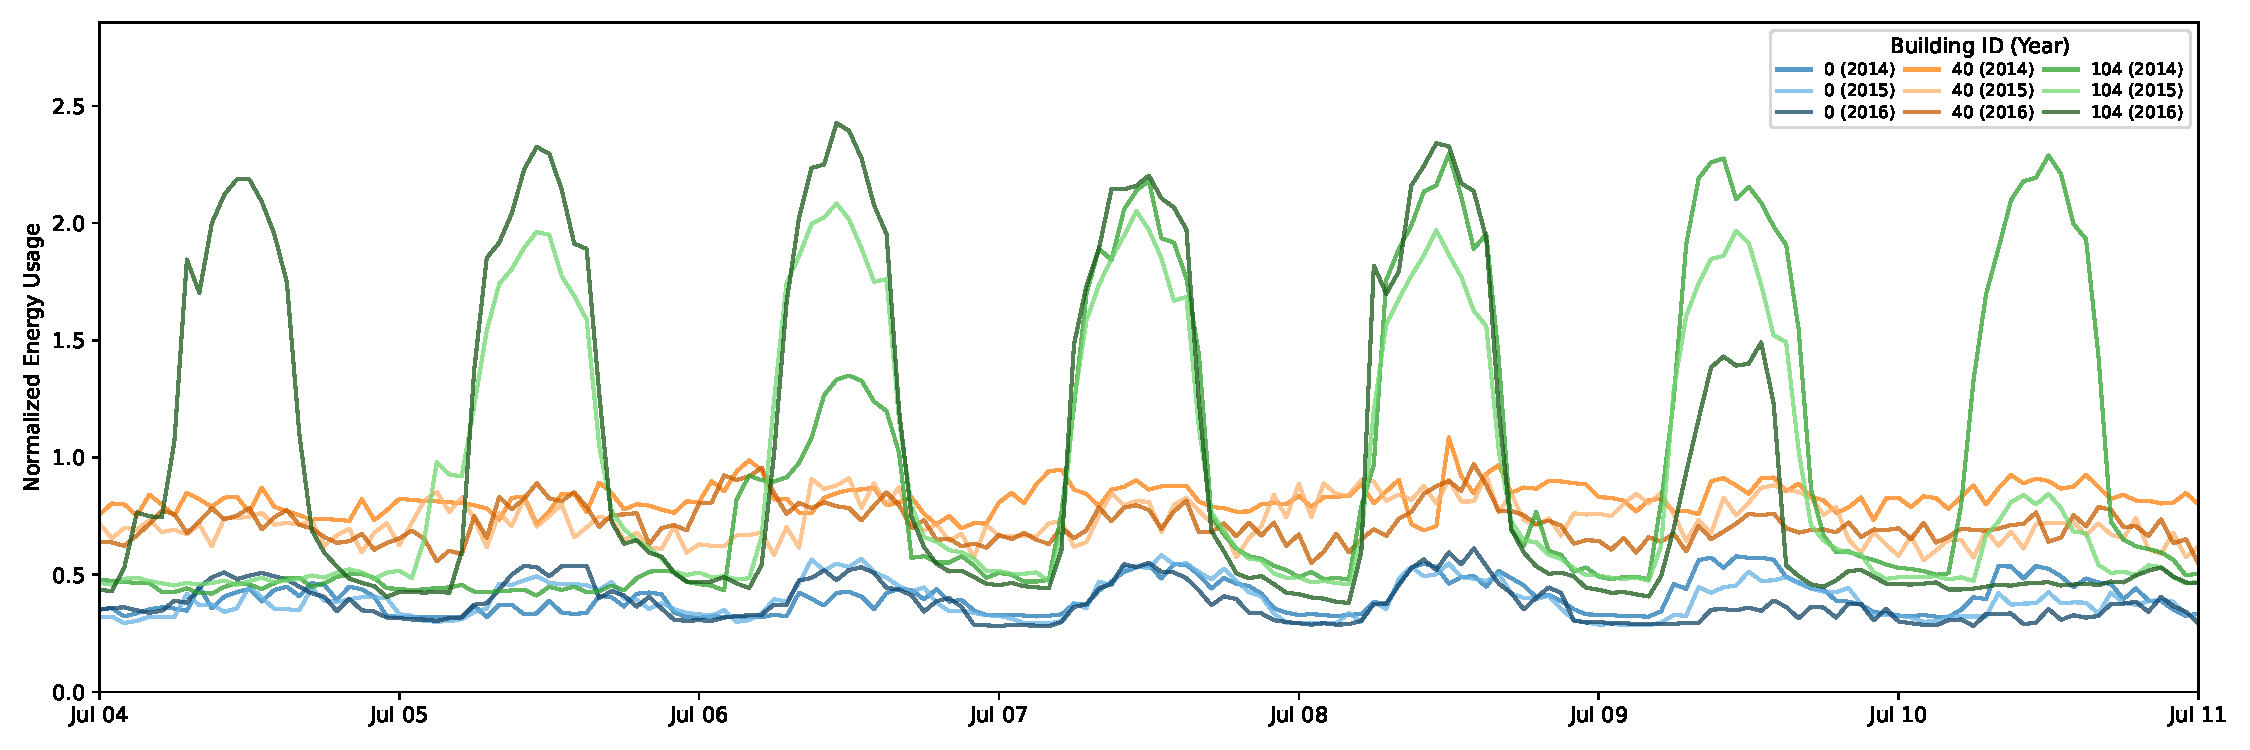
\includegraphics[width=\linewidth]{districts_load_data_summer.pdf} \label{fig:districts-summer-loads}
    }

    \subfloat[Winter.]{
        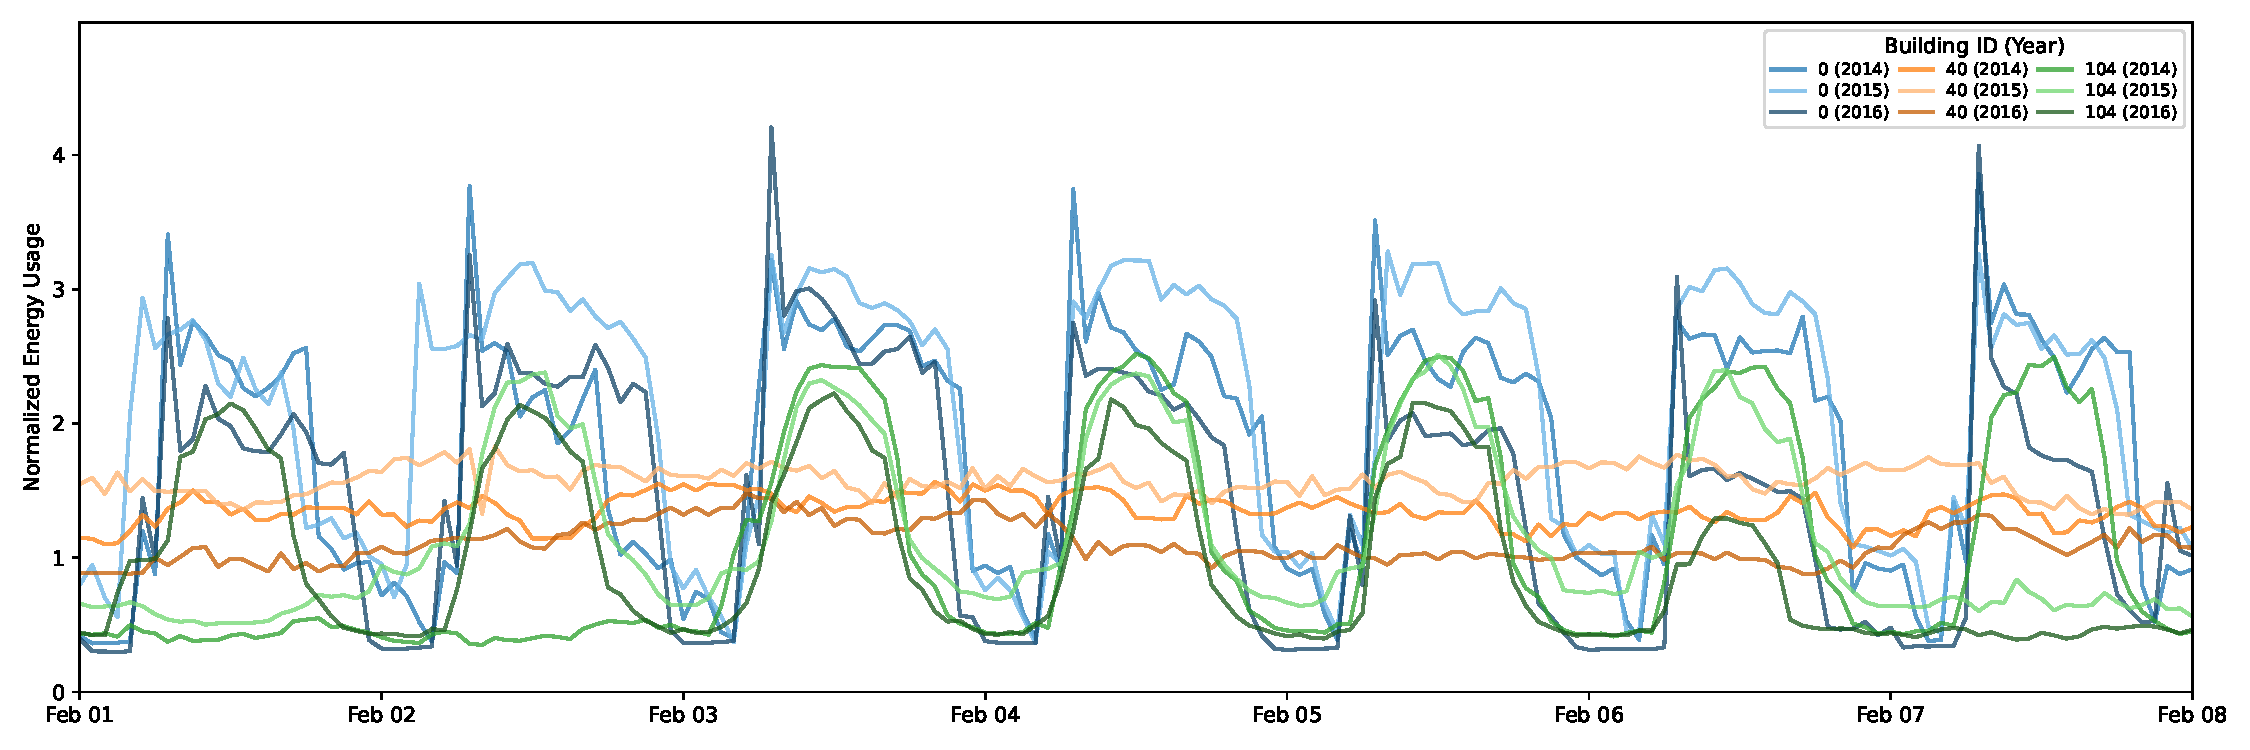
\includegraphics[width=\linewidth]{districts_load_data_winter.pdf} \label{fig:districts-winter-loads}
    }
    \vspace*{-0.2cm}
    \caption{Example electricity load profiles, representing buildings with electrified heating.} \label{fig:districts-example-load-data}
    \vspace{0.1cm}
    \small{\textit{The complete set of electrified building load profiles considered in the case study can be view interactively} \href{https://mal84emma.github.io/Building-Design-VoI/load_dataset_plot.html}{\textbf{here}}.}
\end{figure}


\subsection{Probabilistic models of uncertain building electrical load \& measurement via monitoring} \label{sec:districts-prob}

% Note that we are using data to model complex uncertainties in funcational variables (load profiles), which we parameterize
% Specifically looking at reduction in uncertainty in hourly load profile (important because of peaks), corresponding to data collected from building monitoring system
% Explain derivation of probabalistic models, may need to include figures (in appendix?)
% Highlight posterior representing *practical* measurement - derived from real data

A probabilistic model of the uncertain electricity load of a building is constructed from the data. The functional data variables representing building load are parameterized to provide a simple statistical representation that allows the importance of different characteristics of electrical load to be studied. Four parameters are used to specify the load profiles, two representing the shape of the profile (\texttt{type} and \texttt{year}), and two representing the scale of electricity usage (\texttt{mean} and \texttt{peak}).

The probabilistic models of profile shape are taken directly from data. The parameter \texttt{type} is used to represent the broad patterns of energy usage exhibited by a building, which derive largely from its usage type, e.g. laboratory, teaching, office, or a mix thereof. It is taken as a categorical variable denoting which building in the case study dataset the load profile data is taken from. All buildings are assumed equally likely,
\begin{equation} \label{eqn:id-model}
    \texttt{type} \sim \mathcal{U}\left(\lbrace \text{available buildings} \rbrace\right)
\end{equation}
The parameter \texttt{year} is used to represent the inherent randomness in building energy usage due to factors that cannot be known in advance, such as occupant behaviour and weather. It is taken as a categorical variable denoting the year from which the load profile data is taken, which are all assumed equally likely,
\begin{equation} \label{eqn:year-model}
    \texttt{year} \sim \mathcal{U}\left(\lbrace 2012,\ldots,2017 \rbrace\right)
\end{equation}
Load monitoring is assumed to provide knowledge of the broad energy usage patterns of a building, i.e. perfect information for the parameter \texttt{type} and no information for \texttt{year}.

Probabilistic models for the scale of electricity usage are determined from the statistics of the available load data. The prior model of mean building load is taken to be,
\begin{equation} \label{eqn:mean-model}
    \texttt{mean} \sim \mathcal{N}(100,25)
\end{equation}
representing a $\pm50\%$ uncertainty in a design load of 100kW.

The prior model of peak building load is taken to be,
\begin{equation} \label{eqn:peak-model}
    \texttt{peak} \sim \mathcal{U}(200,400)
\end{equation}
which is fit using the annual peak loads from the dataset.

In a practical building, load monitoring provides an uncertain/imperfect estimate of the mean and peak building load, as there is year-on-year variation in these values that cannot be predicted in advance. The likelihood models for the precision of mean and peak load measurements (estimates) from building monitoring are taken to be Gaussian, with measurement errors determined using the year-on-year variations observed in the load dataset, i.e. the likelihood of obtaining a measurement value is,
\begin{equation}
    z|\theta \sim \mathcal{N}(\theta,\varepsilon\theta)
\end{equation}
with $\varepsilon = 0.1$ for \texttt{mean}, and $\varepsilon = 0.075$ for \texttt{peak}.\\

The prior probabilistic models of the parameters describing the building electricity load profiles, and the likelihood models for measurements made via building monitoring are summarized in Table \ref{tab:districts-prob-models}. Where necessary, the corresponding posterior distributions are modelled using \texttt{Stan} \citep{carpenter2017StanProbabilisticProgramming}.

The probabilistic models of electrical load are taken to be the same for all buildings in the district, with the parameters \texttt{type}, \texttt{mean}, and \texttt{peak} independent for each building. The \texttt{year} parameter is the common to all buildings (sampled once for the district in each scenario). This is done to ensure that correlations in the timing of energy usage between buildings are properly captured, as building energy usage is driven by common externalities across the district, for example outdoor temperature which affects heating load. These correlations in building loads are important for correctly representing the overall energy usage behaviour of the district. For example, the relative timing of peaks in building load determines the district peak load, and so the required grid connection capacity.

Samples are drawn from the building load distributions (either prior or posterior) by sampling the four parameters (\texttt{type}, \texttt{year}, \texttt{mean}, \texttt{peak}) using their probabilistic models, retrieving the constructed electrified heating load data for the sampled building (\texttt{type}) and year (see Fig. \ref{fig:districts-example-load-data}), and scaling the profile to the sampled mean and peak load values.

\vfill

\begin{table}[h]
    \centering
    \renewcommand{\arraystretch}{1.25}
    \centerline{
    \begin{tabular}{c|cccc} \toprule \toprule
        Parameter & Prior model & Prior params & Measurement model & Msr. params \\
        \midrule \midrule
        \texttt{type} & \multirow{2}{*}{Discrete uniform} & $\{ \text{building ids} \}$ & Exact (perfect info) & -- \\
        \texttt{year}* & & $\{ \text{data years} \}$ & None (no info) & -- \\
        \midrule
        \texttt{mean} & Gaussian & \makecell{$\mu=\SI{100}{kW}$\\$\sigma=\SI{25}{kW}$} & \multirow{2}{*}{\makecell{Gaussian imprecision\\(imperfect info)\\[1ex]$z|\theta \sim \mathcal{N}(\theta,\varepsilon\theta)$}} & $\varepsilon = 0.1$ \\[2ex]
        \texttt{peak} & Continuous uniform & \makecell{$\min=\SI{200}{kW}$\\$\max=\SI{400}{kW}$} & & $\varepsilon = 0.075$ \\
        \bottomrule \bottomrule
    \end{tabular}
    }
    \smallskip
    \caption{Probabilistic models of parameters describing uncertain building load, and their measurement via monitoring.}
    \vspace*{-0.1cm}
    {\footnotesize *\textit{Parameter common to all buildings in the district}}
    \label{tab:districts-prob-models}
\end{table}

\newpage

The prior probabilistic model of building electrical load is visualised in Fig. \ref{fig:districts-load-dist}. The mean load profile is indicated in black, with confidence intervals of $\pm 1 \text{ s.d.}$, $\pm 2 \text{ s.d.}$, and the range ($\min$ to $\max$), indicated in successively lighter shades of gray. A set of load profiles sampled from the distribution are traced in blue.

Fig. \ref{fig:districts-post-load-dist} illustrates the posterior distribution of building load for an example load profile measurement obtained by building monitoring (indicated in red). Load profiles sampled from the posterior distribution are traced in green. The confidence intervals of the prior distribution, from Fig. \ref{fig:districts-load-dist}, are underlaid for comparison. The tighter clustering of the profiles sampled from the posterior compared to that for the prior samples in Fig. \ref{fig:districts-load-dist} demonstrates the reduction in building load uncertainty achieved by monitoring.\\

\newcommand{\tsfw}{1}
\begin{figure}[!h]
    \centering
    \subfloat[Summer.]{
        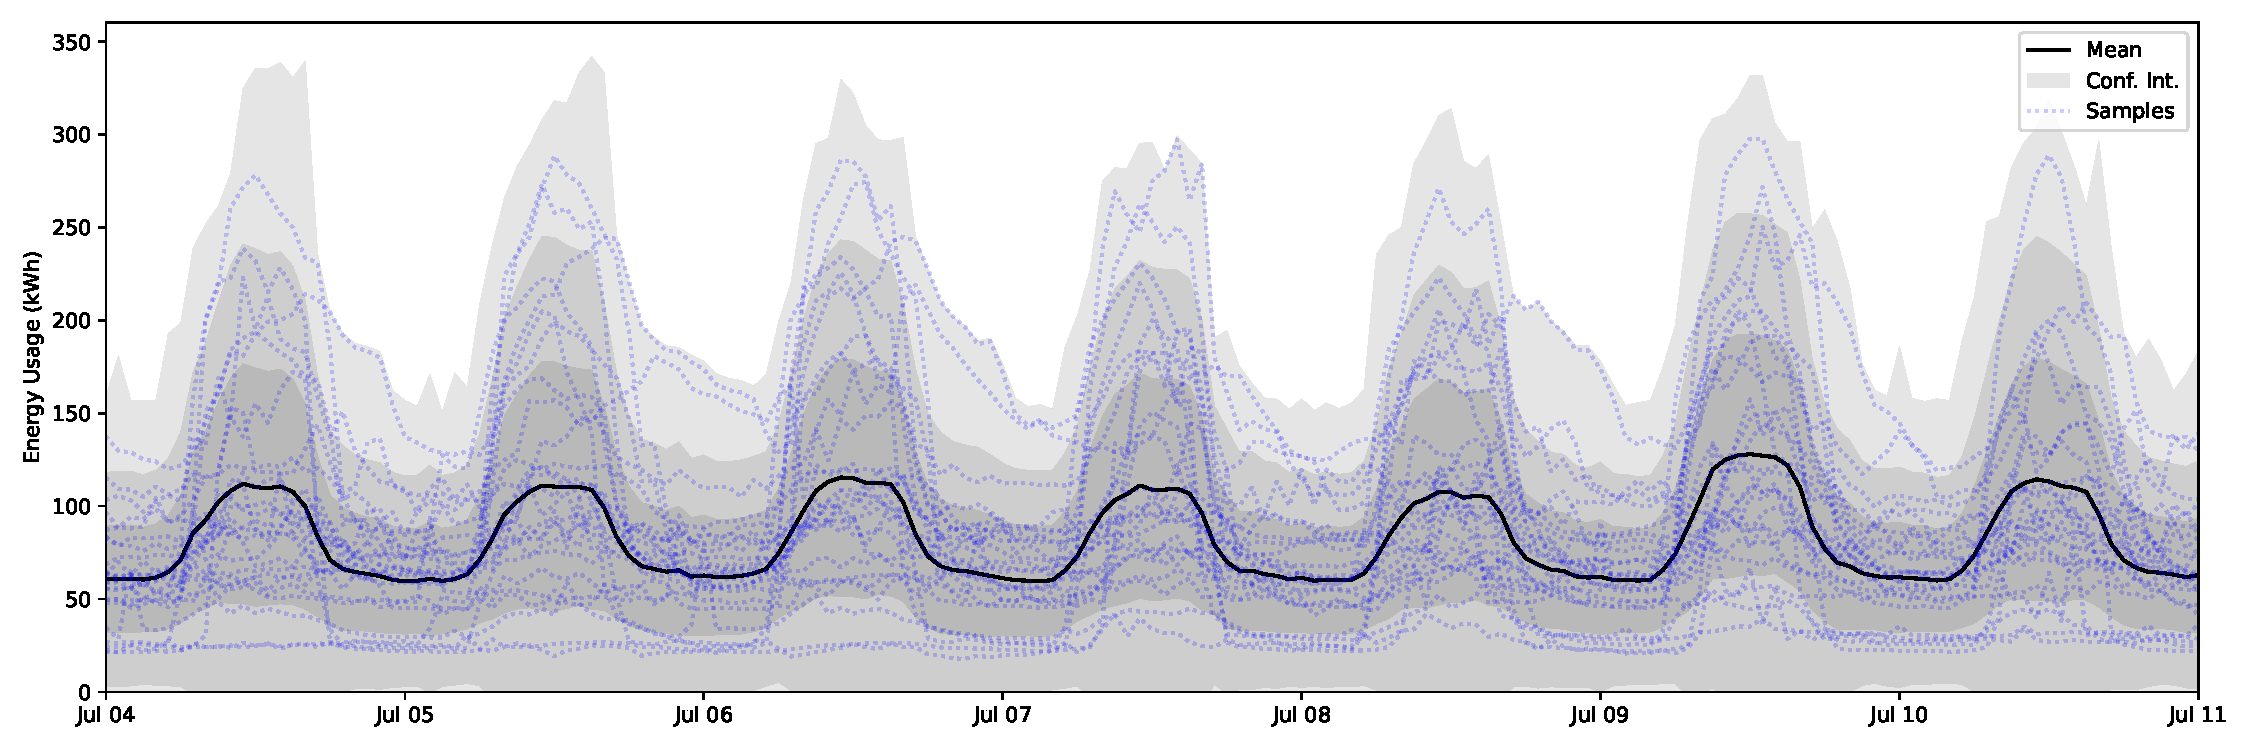
\includegraphics[width=\tsfw\linewidth]{districts_prior_load_dist_summer.pdf} \label{fig:districts-summer-dist}
    }

    \subfloat[Winter.]{
        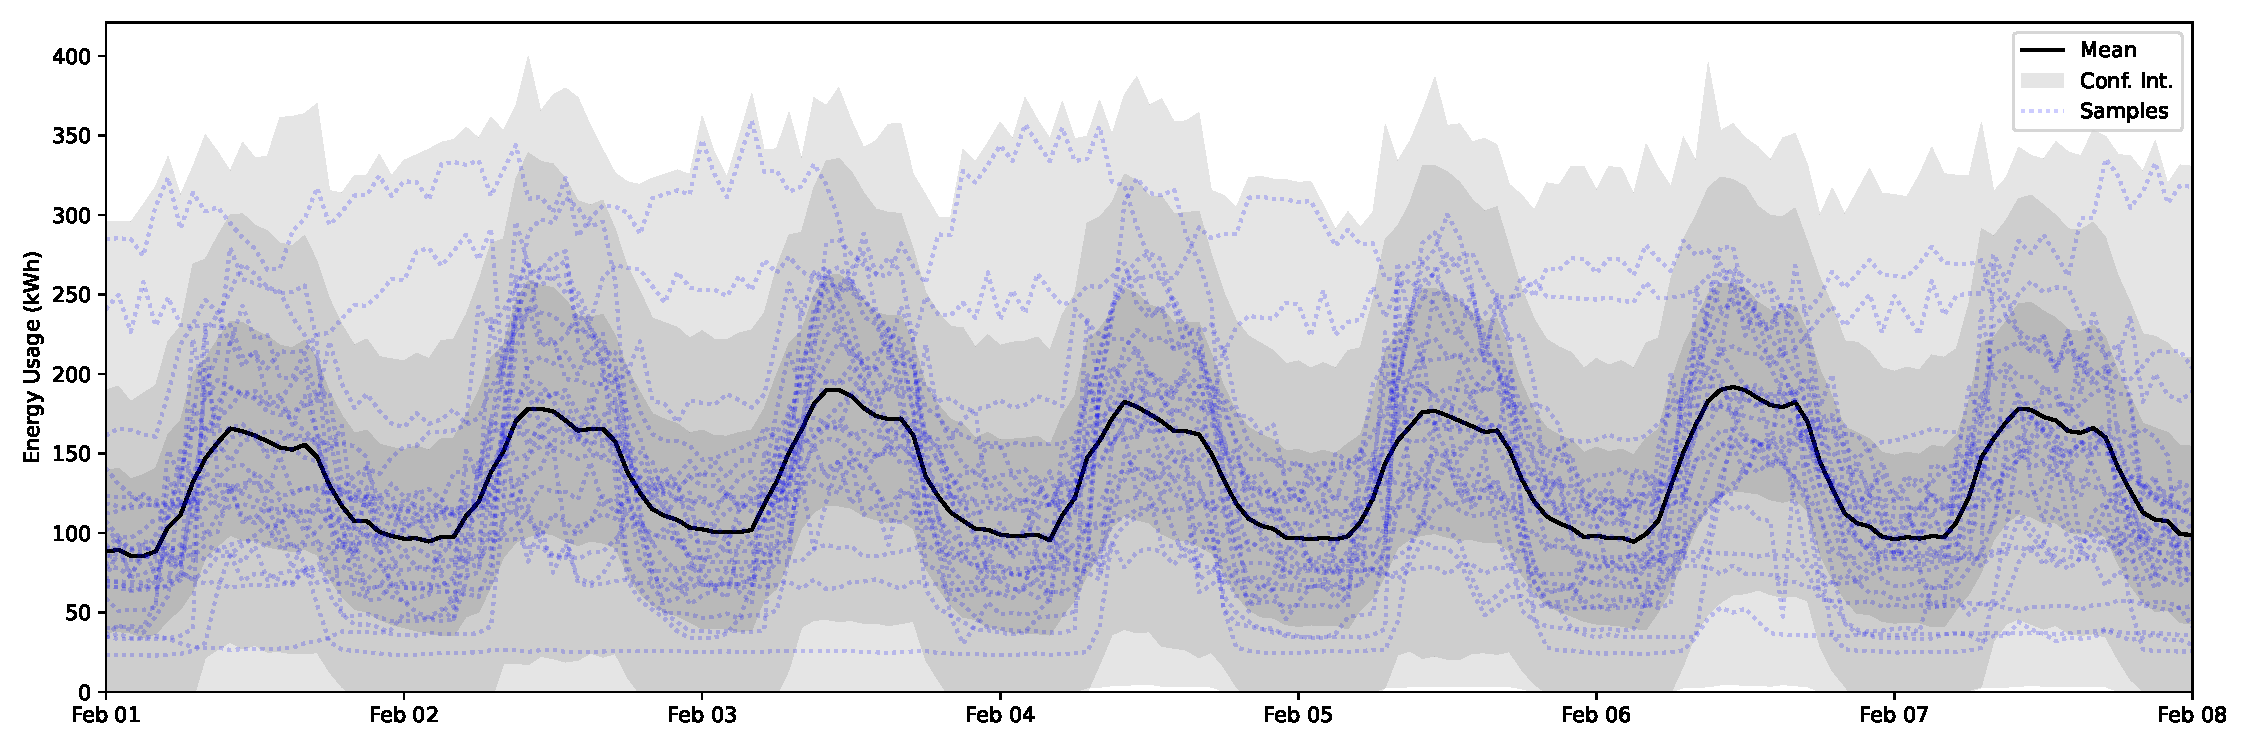
\includegraphics[width=\tsfw\linewidth]{districts_prior_load_dist_winter.pdf}
        \label{fig:districts-winter-dist}
    }
    \vspace*{-0.2cm}
    \caption{Visualisation of prior probabilistic model of uncertain building load, with profiles sampled from distribution.} \label{fig:districts-load-dist}
\end{figure}

\begin{figure}[ht]
    \centering
    \subfloat[Summer.]{
        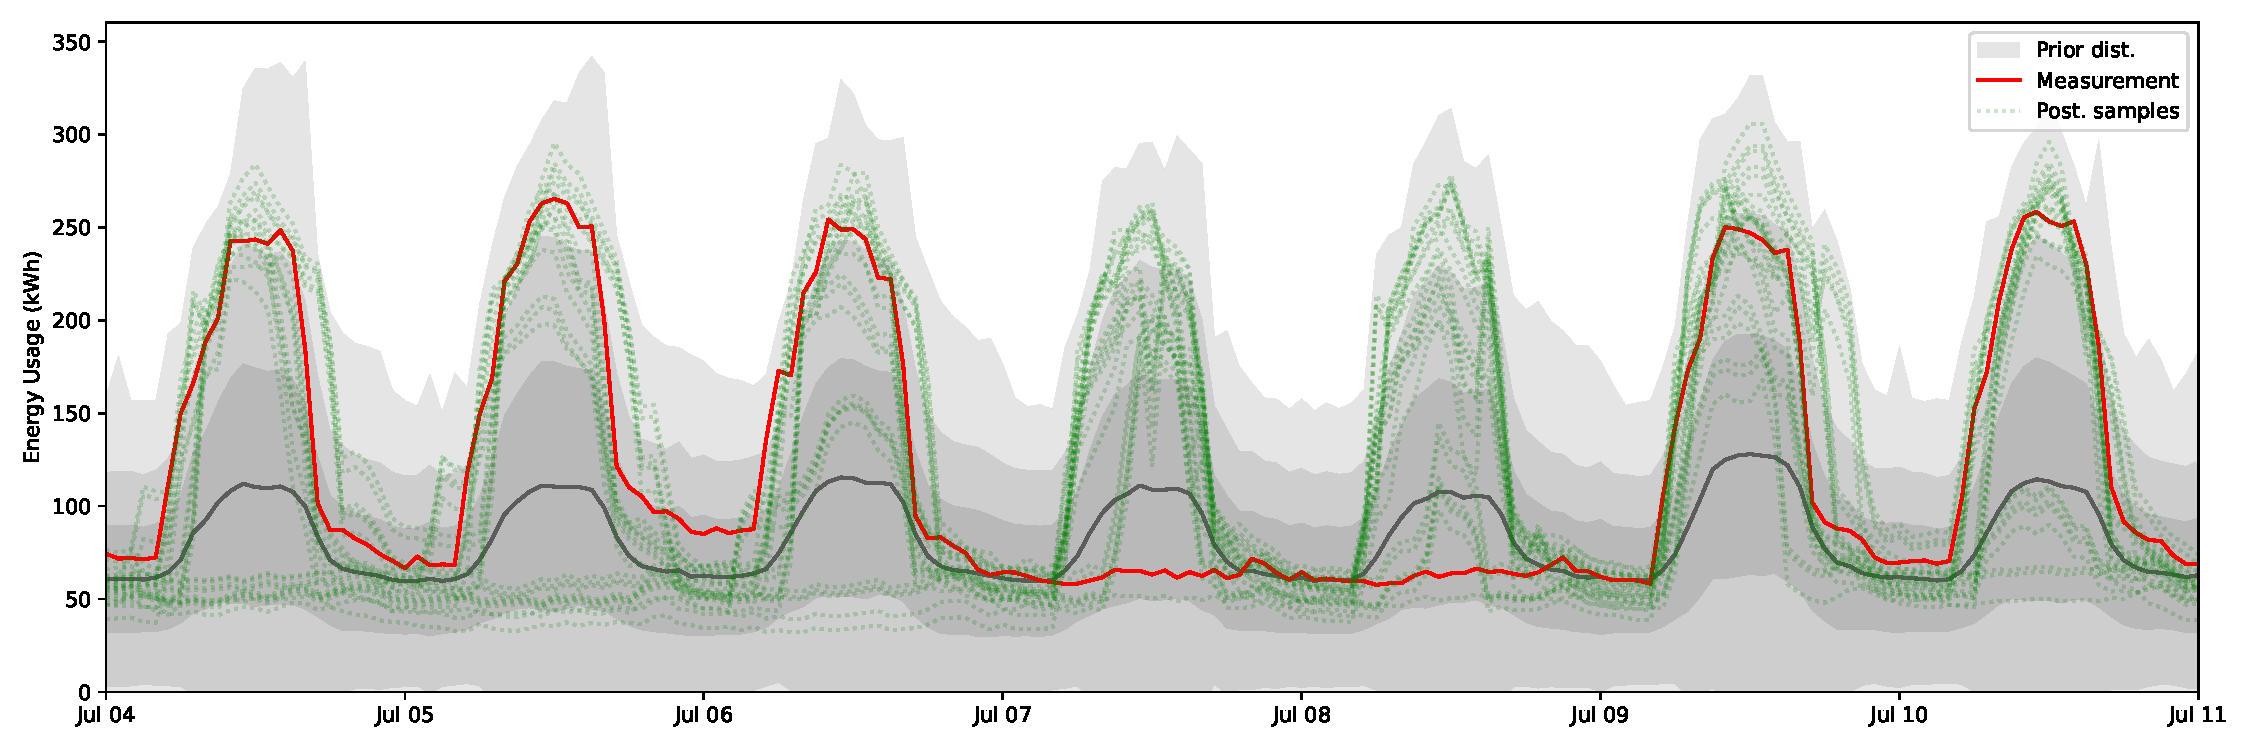
\includegraphics[width=\tsfw\linewidth]{districts_post_load_dist_summer.pdf} \label{fig:districts-summer-post-dist}
    }

    \subfloat[Winter.]{
    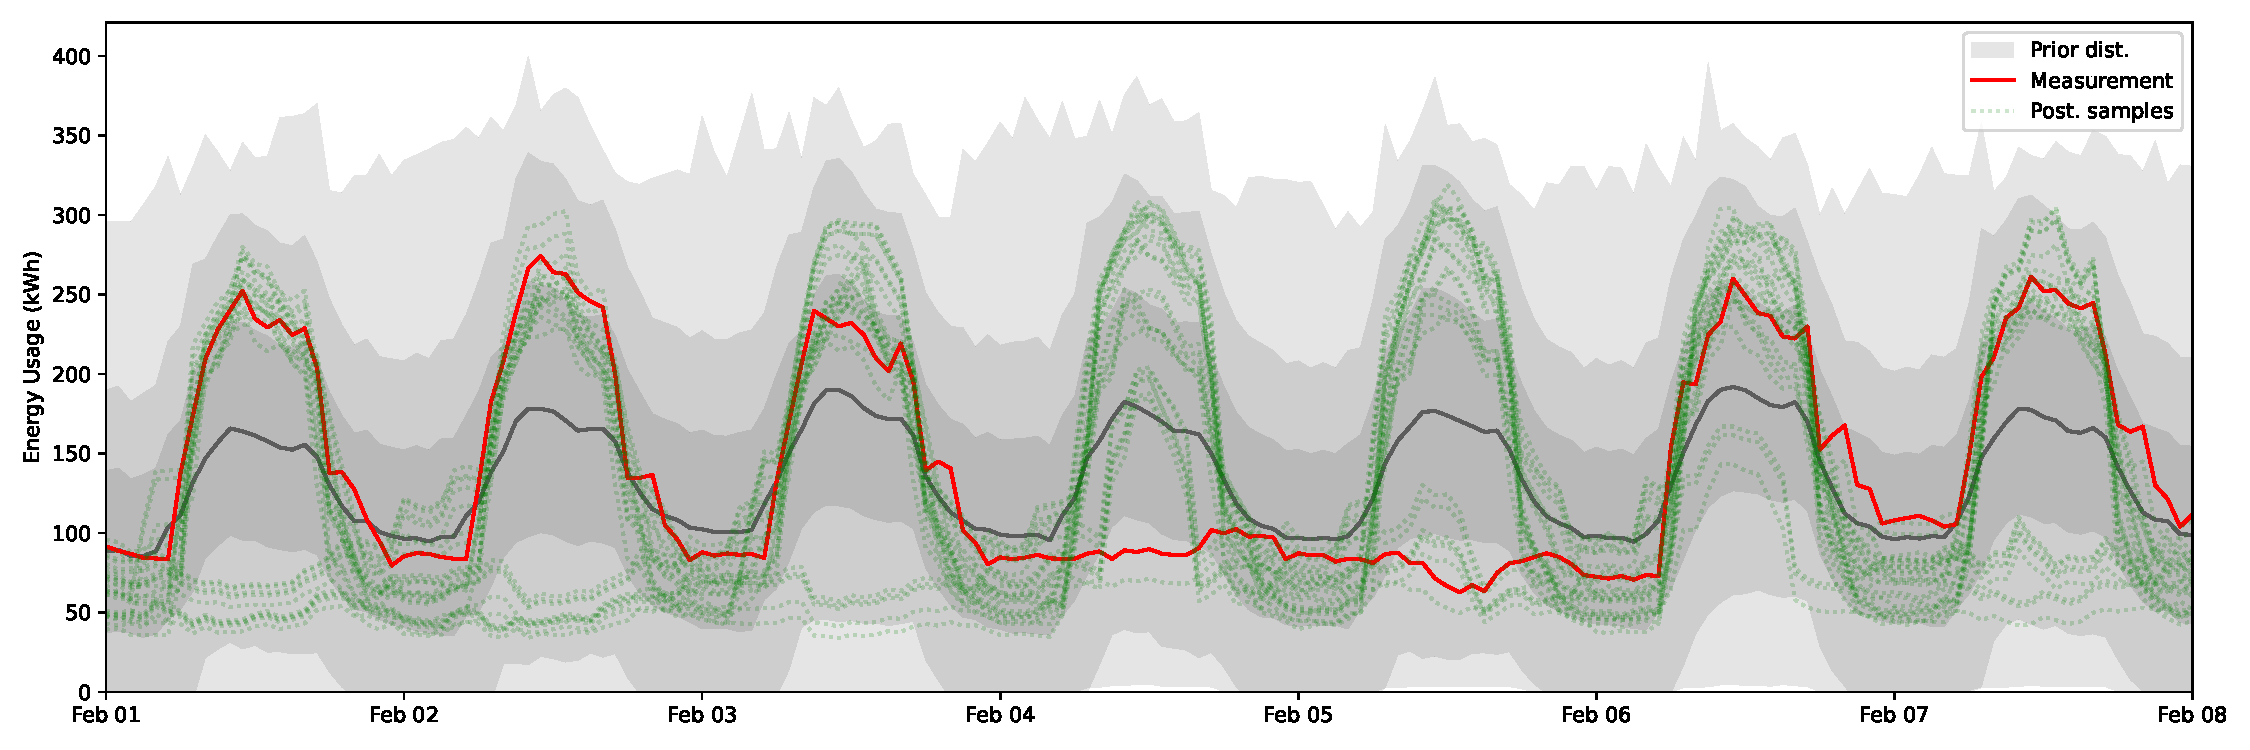
\includegraphics[width=\tsfw\linewidth]{districts_post_load_dist_winter.pdf}
    \label{fig:districts-winter-post-dist}
    }
    \caption{Visualisation of posterior probabilistic model of building load for example measurement.} \label{fig:districts-post-load-dist}
\end{figure}


\clearpage
\subsection{Stochastic Programming for system sizing} \label{sec:districts-SP}

% mention why Stochastic Programming chosen for system design (popular choice and well suited for systems with lots of decision variables - e.g. district energy systems)
% remember to discuss scenario reduction - need to use simple metrics (instead of op. results) as scenario space is combinatorial (cite Bryn's thesis)
% explain form of costs (grid connection costs from DUoS charges)
% comment that SP does not provide accurate estimate of true system cost due to: safety factor, over-optimism induced by excessive information availability (leading to need for safety factor)

For the case study, Stochastic Programming is used as a policy to optimize the sizing of solar PV, battery storage units, and grid connection capacity, to determine district energy system designs that (attempt to) minimize the expected total system cost, accounting for uncertainty in electrical load and solar generation. Stochastic Programming (specifically linear scenario programming) is chosen as the modelling and optimization methodology due to its computational efficiency for problems with large numbers of decision variables, and its resulting prevalent use in the current literature for designing district- and national-scale energy systems \citep{decarolis2017FormalizingBestPractice,pickering2019DistrictEnergySystem,yue2018ReviewApproachesUncertainty,2024OpenEnergyModelling,yang2015MILPMixedInteger}.

A linearized model of the electrical behaviour of the district energy system is used. A schematic of the energy flows within the district energy system model is provided in Fig. \ref{fig:districts-energy-system}. This allows the design optimization task to be formulated as a Linear Program, which is presented in Eq. \ref{eq:districts-SP}, with Table \ref{tab:districts-LP-params} providing descriptions of the parameters. The model formulation uses the same form of constraints to represent energy system behaviour as state-of-the-art models such as \citep{pfenninger2018CalliopeMultiscaleEnergy} and \citep{brown2018PyPSAPythonPower}.\\

%\newpage
\begin{figure}[h]
    \centering
    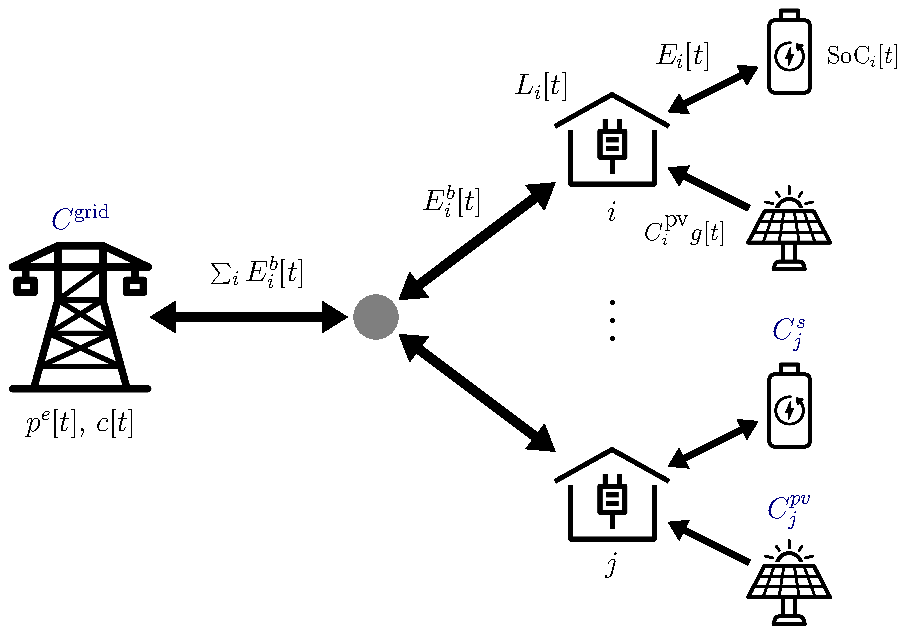
\includegraphics[width=0.8\linewidth]{districts_sys-diagram.pdf}
    \caption{Energy flow schematic for case study district energy system.}
    {\scriptsize Operational variables are indicated in black, capacity variables are indicated in blue. (Icon credits: \href{https://thenounproject.com/symbolon/}{Symbolon})}
    \label{fig:districts-energy-system}
\end{figure}

\begin{subequations} \label{eq:districts-SP}
    \begin{align}
        \addtocounter{equation}{-1}
        \begin{split}
        \text{min} & \qquad \mathlarger{\gamma} \:\: \mathlarger{\mathlarger{\sum}}_m \: \rho_m \vast( \mathlarger{\sum}_t \Bigg( \underbrace{p^e[t] \sum_i \left( \max \left[ 0,\, E_{i,m}^b[t] \right] \right)}_{\text{electricity cost}} + \, \underbrace{p^c \, c[t] \, \max \Bigg[ 0,\, \sum_i E_{i,m}^b[t] \Bigg]}_{\text{carbon cost}} \Bigg) \\[1ex]
        & \hspace{4cm} + \:\: \underbrace{p^{\textrm{grid}}_{\textrm{excess}} \max \Bigg[0, \max_t \bigg[ \Big| \sum_i E_{i,m}^b[t] \Big| \bigg]\Big/\Delta t - C^{\textrm{grid}}/\text{FoS} \Bigg]}_{\text{grid excess cost}} \vast)\\[1ex]
        & \hspace{2cm} + \underbrace{\mathlarger{\mathlarger{\sum}}_i \bigg( p^{\textrm{s}} C^{\textrm{s}}_i + p^{\textrm{pv}} C^{\textrm{pv}}_i \bigg)}_{\text{capital cost}} + \underbrace{\vphantom{\mathlarger{\sum}_i} \mathlarger{\gamma} \: p^{\textrm{grid}} C^{\textrm{grid}} \:}_{\text{grid connection cost}}
        \end{split} \label{eq:districts-lp} \\[\eqnskip]%%
        \text{over} & \qquad C^{\textrm{s}}_i,\, C^{\textrm{pv}}_i,\, C^{\textrm{grid}},\, E_{i,m}[t],\, \textrm{SoC}_{i,m}[t{+}1] \quad \forall \: i,\, m,\, t \tag*{} \\[\eqnskip]
        \text{subject to} & \qquad \textrm{SoC}_{i,m}[t{+}1] = \textrm{SoC}_{i,m}[t] + \sqrt{\eta_i} \left[E_{i,m}[t]\right]^{+} - 1/\sqrt{\eta_i} \left[\, E_{i,m}[t] \right]^{-} \label{eq:districts-dynamics-constraint} \\[\smalleqnskip]
        & \qquad -P^{\textrm{max}}_i \Delta t \leq E_{i,m}[t] \leq P^{\textrm{max}}_i \Delta t \label{eq:districts-power-constraint} \\[\smalleqnskip]
        & \qquad 0 \leq \textrm{SoC}_{i,m}[t{+}1] \leq C^{\textrm{s}}_i \label{eq:districts-energy-constraint} \\[\smalleqnskip]
        & \qquad C^{\textrm{s}}_i,\, C^{\textrm{pv}}_i,\, C^{\textrm{grid}} \geq 0 \\[\smalleqnskip]
        & \qquad P^{\textrm{max}}_i = \delta C^{\textrm{s}}_i \label{eq:districts-power-capacity} \\[\smalleqnskip]
        & \qquad \textrm{SoC}_{i,m}[0] = \textrm{SoC}^0 C^{\textrm{s}}_i \label{eq:districts-initial-conditions} \\[\smalleqnskip]
        & \qquad E^b_{i,m}[t] = L_{i,m}[t] - C^{\textrm{pv}}_i g_m[t] + E_{i,m}[t] \label{eq:districts-aggregation-constraint} \\[\eqnskip]%%
        \text{for all} & \qquad i \in [0,B{-}1], \: t \in [0,T{-}1], \: m \in [0,M{-}1] \tag*{}
    \end{align}
\end{subequations}

\begin{table}[hp]
    \centering
    \renewcommand{\arraystretch}{1.25}
    \centerline{
    \begin{tabularx}{1.05\linewidth}{ccX} \toprule \toprule
        Parameter & Units & \multicolumn{1}{>{\centering\arraybackslash}c}{Description} \\
        \midrule \midrule
        \multicolumn{3}{>{\centering\arraybackslash}l}{\small \quad Decision variables} \\
        $C^{\textrm{s}}_i$ & kWh & Energy capacity of battery unit in building $i$ \\
        $C^{\textrm{pv}}_i$ & kWp & Peak power capacity of solar PV unit in building $i$ \\
        $C^{\text{grid}}$ & kW & Contracted power capacity of grid connection \\
        $E_{i,m}[t]$ & kWh & Energy \textit{intake} to battery unit in building $i$ at time $t$ in scenario $m$ \\
        $\textrm{SoC}_{i,m}[t]$ & kWh & State-of-charge of battery unit in building $i$ at time $t$ in scenario $m$ \\
        \midrule
        \multicolumn{3}{>{\centering\arraybackslash}l}{\small \quad Derived variables} \\
        $E^b_{i,m}[t]$ & kWh & Net energy flow \textit{into} building $i$ at time $t$ in scenario $m$ \\
        $P^{\textrm{max}}_i$ & kW & Power capacity of battery unit in building $i$ \\
        \midrule
        \multicolumn{3}{>{\centering\arraybackslash}l}{\small \quad Parameters (data)} \\
        $\gamma$ & yrs & System lifetime \\ %(multiple of operational period, $T$) \\
        $\Delta t$ & hrs & Time step of simulation data \\
        $\rho_m$ & -- & Probability of scenario $m$ \\
        $\delta$ & kW/kWh & Discharge ratio of battery units (power capacity/energy capacity) \\
        $\textrm{SoC}^0$ & -- &  Initial state-of-charge of battery units (fraction of capacity) \\
        $\eta_i$ & -- & Round-trip efficiency of battery unit in building $i$ \\
        $L_{i,m}[t]$ & kWh & Electrical demand of building $i$ at time $t$ in scenario $m$ \\
        $g_m[t]$ & kW/kWp & Normalised generation power from solar PV at time $t$ in scenario $m$ \\
        $p^e[t]$ & £/kWh & Grid electricity price at time $t$ \\
        $p^c$ & £/kgCO$_2$ & Nominal carbon price \\
        $c[t]$ & kgCO$_2$/kWh & Carbon intensity of grid electricity at time $t$ \\
        $p^{\textrm{s}}$ & £/kWh & Unit price of battery storage \\
        $p^{\textrm{pv}}$ & £/kWp & Unit price of solar PV \\
        $p^{\text{grid}}$ & £/kW & Price of contracted grid connection capacity (over operational period) \\
        $p^{\text{grid}}_{\text{excess}}$ & £/kW & Excess charge for exceeding contracted grid capacity (over operational period) \\
        $\text{FoS}$ & -- & Factor of safety for grid connection capacity \\
        \bottomrule \bottomrule
    \end{tabularx}
    }
    \smallskip
    \caption{Description of Stochastic Program variables \& parameters.} \label{tab:districts-LP-params}
\end{table}
\hfill

\newpage
The design optimization seeks to minimize as its objective the average total lifetime system cost over a set of $M$ scenarios for the district of $B$ buildings, operated for period of length $T$. This total system cost is comprised of: the capital cost of solar PV and battery units in the buildings, the cost of electricity purchased from the grid (metered per building), the cost of carbon emissions associated with used grid electricity (for the overall district), and the cost of grid usage.
This optimization is subject to energy conservation\footnote{$[\,\cdot\,]^+$ and $[\,\cdot\,]^-$ represent the positive and negative parts of the argument respectively.} (Eq. \ref{eq:districts-dynamics-constraint}) and capacity (Eq. \ref{eq:districts-power-constraint} \& Eq. \ref{eq:districts-energy-constraint}) constraints for operation within each scenario $m$.

The cost of grid usage is modelled following the form of Distributed Use of Service (DUoS) connection capacity charges, which are the costs charged to large electricity consumers connected to the distribution network in the UK \citep{acha2022ModellingUKElectricity,frontiereconomics2022NetworkTariffsEnergy}. These consumers must request a `contracted' connection capacity from the distribution operator, for which they are charged a cost per unit of connection capacity (£/kVA). If during operation a consumer draws power from the grid exceeding this contracted capacity, they are charged an additional cost for each kVA that their peak power draw exceeds the contracted capacity. Exaggerated grid charges (compared to current values) are used to represent the pressure on network connection capacity caused by future heat electrification.

As Linear Programs simultaneously optimize over all operational variables, they assume that the district energy system is operated with perfect foresight. This leads to underestimation of the system operational costs, as the battery units within the modelled energy system are scheduled more effectively than could be achieved in practice, reacting to and avoiding future costs which could not be foreseen. This is particularly important for the grid excess costs which depend on peak grid load values that are greatly influenced by the perfect foresight assumption. To account for this underestimation of grid usage in the design model, a factor of safety ($\text{FoS}$) is introduced into the grid excess cost. This $\text{FoS}$ was calibrated using preliminary experiments, and was found to greatly reduce the overall cost of designs, as evaluated using the operational simulations introduced in the following section. % can be easily shown if reviewer asks

The Stochastic Program requires samples (scenarios) to be drawn from the probability space of electrical load profiles for each building in the district. As a result, the space of possible load scenarios is extremely large. However, due to the cubic computational complexity of Linear Programming, only a small number of scenarios can be tractably included in the Scenario Optimization. Therefore, after load profile samples are drawn, scenario reduction \citep{heitsch2003ScenarioReductionAlgorithms,gioia2023ScenarioReducer} is performed to select a reduced set of 10 scenarios\footnote{The maximum number which could be used by the Stochastic Program given the available computational budget.} that are statistically representative of the initial sample. A large initial sample must be considered to adequately cover the probability space of district loads. Therefore state-of-the-art scenario reduction methods which optimize each scenario individually, and use the resulting distribution of costs as the reduction metric \citep{pickering2019PracticalOptimisationDistrict} are intractable. Instead, computationally cheap scenario metrics must be used. The mean, maximum, and standard deviation of the aggregate electrical load for the district are chosen as the metrics for scenario reduction, as simple features representing the shape and scale of the district electricity load.

The parameter values used for all experiments are detailed in \ref{app:districts-case-study-params}.


\subsection{Evaluation of operational cost of system designs via simulation} \label{sec:districts-sims}

% Explain why we want to use the simulation for evals (SP doesn't accurately estimate cost, due to; over-optimism, small sample size) - highlight design vs operation distinction from SP
% Receeding horizon MPC using same LP as design (reduced FoS), over horizon $\tau$ with perfect forecasts
% Generally SP objectives are not fully reliable (under-estimate costs due to excessive info availability), but in this case adding in the heuristics improves system performance, but means the SP objective is not the actual system cost, so additional eval needed anyway
% Highlight importance of design LP and simulations being mathematically identical (MPC model matches simulator), with the only difference being the quantity of information available for making control decision (omniscience vs finite horizon) - and the objective fn

The objective of the Stochastic Program (SP) provides only an approximation of the expected (mean) total cost of the district energy system. The perfect foresight assumption of the Linear Program model causes underestimation of operating costs, a modelling error which is only partly corrected by the factor of safety. The small number of scenarios which can be considered in the Scenario Optimization due to computational limitations causes statistical error in the estimation of the mean cost.
The combined model and statistical errors could lead to significant inaccuracy in the cost estimates\footnotemark, and so the \glsxtrshort{voi}. To provide more accurate estimations of the true cost of system designs (the decision maker's target utility), the operation of the district energy system is simulated.
\footnotetext{The accuracy of Stochastic Program objective's estimate of total system cost is investigated in \ref{app:districts-cost-accuracy}.}

The CityLearn \citep{vazquez-canteli2019CityLearnV1OpenAI,vazquez-canteli2020CityLearnStandardizingResearch} building energy control framework is used to simulate the behaviour of the district energy system. These simulations provide a more accurate estimate of the operational cost of a system design for a given simulated load scenario. A Model Predictive Control (MPC) scheme is used to schedule battery operation in the simulations. This MPC scheme uses a Linear Programming (LP) formulation with the same form as used for design (Eq. \ref{eq:districts-SP}), however it considers only a single scenario (that being simulated) with perfect forecasts of operational conditions over a 48hr planning horizon. Additionally, a small $\text{FoS}$ is used to prevent numerical errors from the LP solver leading to erroneous exceedance of the grid capacity, calibrated from initial experiments. The simulator is configured with linearized building dynamics, such that the MPC scheme perfectly models the system simulation, and so provides perfect system control with 48hrs of foresight, mirroring the SP used for design, but relaxing the perfect foresight assumption.
As a result, the simulations still underestimate operational costs \citep{langtry2024ImpactDataForecasting}, but this model error is lower than for the SP. As the simulations are computationally cheap, a large number of load scenarios can be simulated, and so the expected cost can be estimated using a large number of Monte Carlo samples (scenarios sampled from the building load distribution), reducing statistical error.


\subsection{Decision problem formulation}

% Briefly but clearly contextualise setup in terms of On-Policy VoI framework
% probabilistic models of uncertain load (pi(theta)) and monitoring measurements (f(z|theta)), SP defines policy, simulations define utility fn - got through section by section and link back to eqn. \ref{eq:districts-OP-VOI}

The case study can be contextualized within the On-Policy \glsxtrshort{voi} framework proposed in \Cref{sec:methodology-on-policy-voi} as follows.

The uncertain parameter in the district energy system, $\theta$, is defined as the electrical load profile (functional variable) in each building, and its probabilistic model, $\pi(\theta)$, is described in parametric form in \Cref{sec:districts-prob} (see Table \ref{tab:districts-prob-models}). The likelihood function, $f(z|\theta)$, describing the uncertainty reduction (imperfect parameter estimates) obtained from building load monitoring, is also described.
A Stochastic Programming model, outlined in \Cref{sec:districts-SP}, is used as a policy, $\mathcal{P}_u$, determining a system design (action) to implement given samples from a distribution of building load profiles (to which scenario reduction is applied due to computational limitations). This policy minimizes an approximation of the expected total system cost (utility). The true system cost (utility, $u$) for a given design is evaluated using simulations of the district energy system with a more realistic control scheme, described in \Cref{sec:districts-sims}. Fig. \ref{fig:districts-method} provides a diagrammatic overview of the methodology.

\begin{figure}[p]
    \centering
    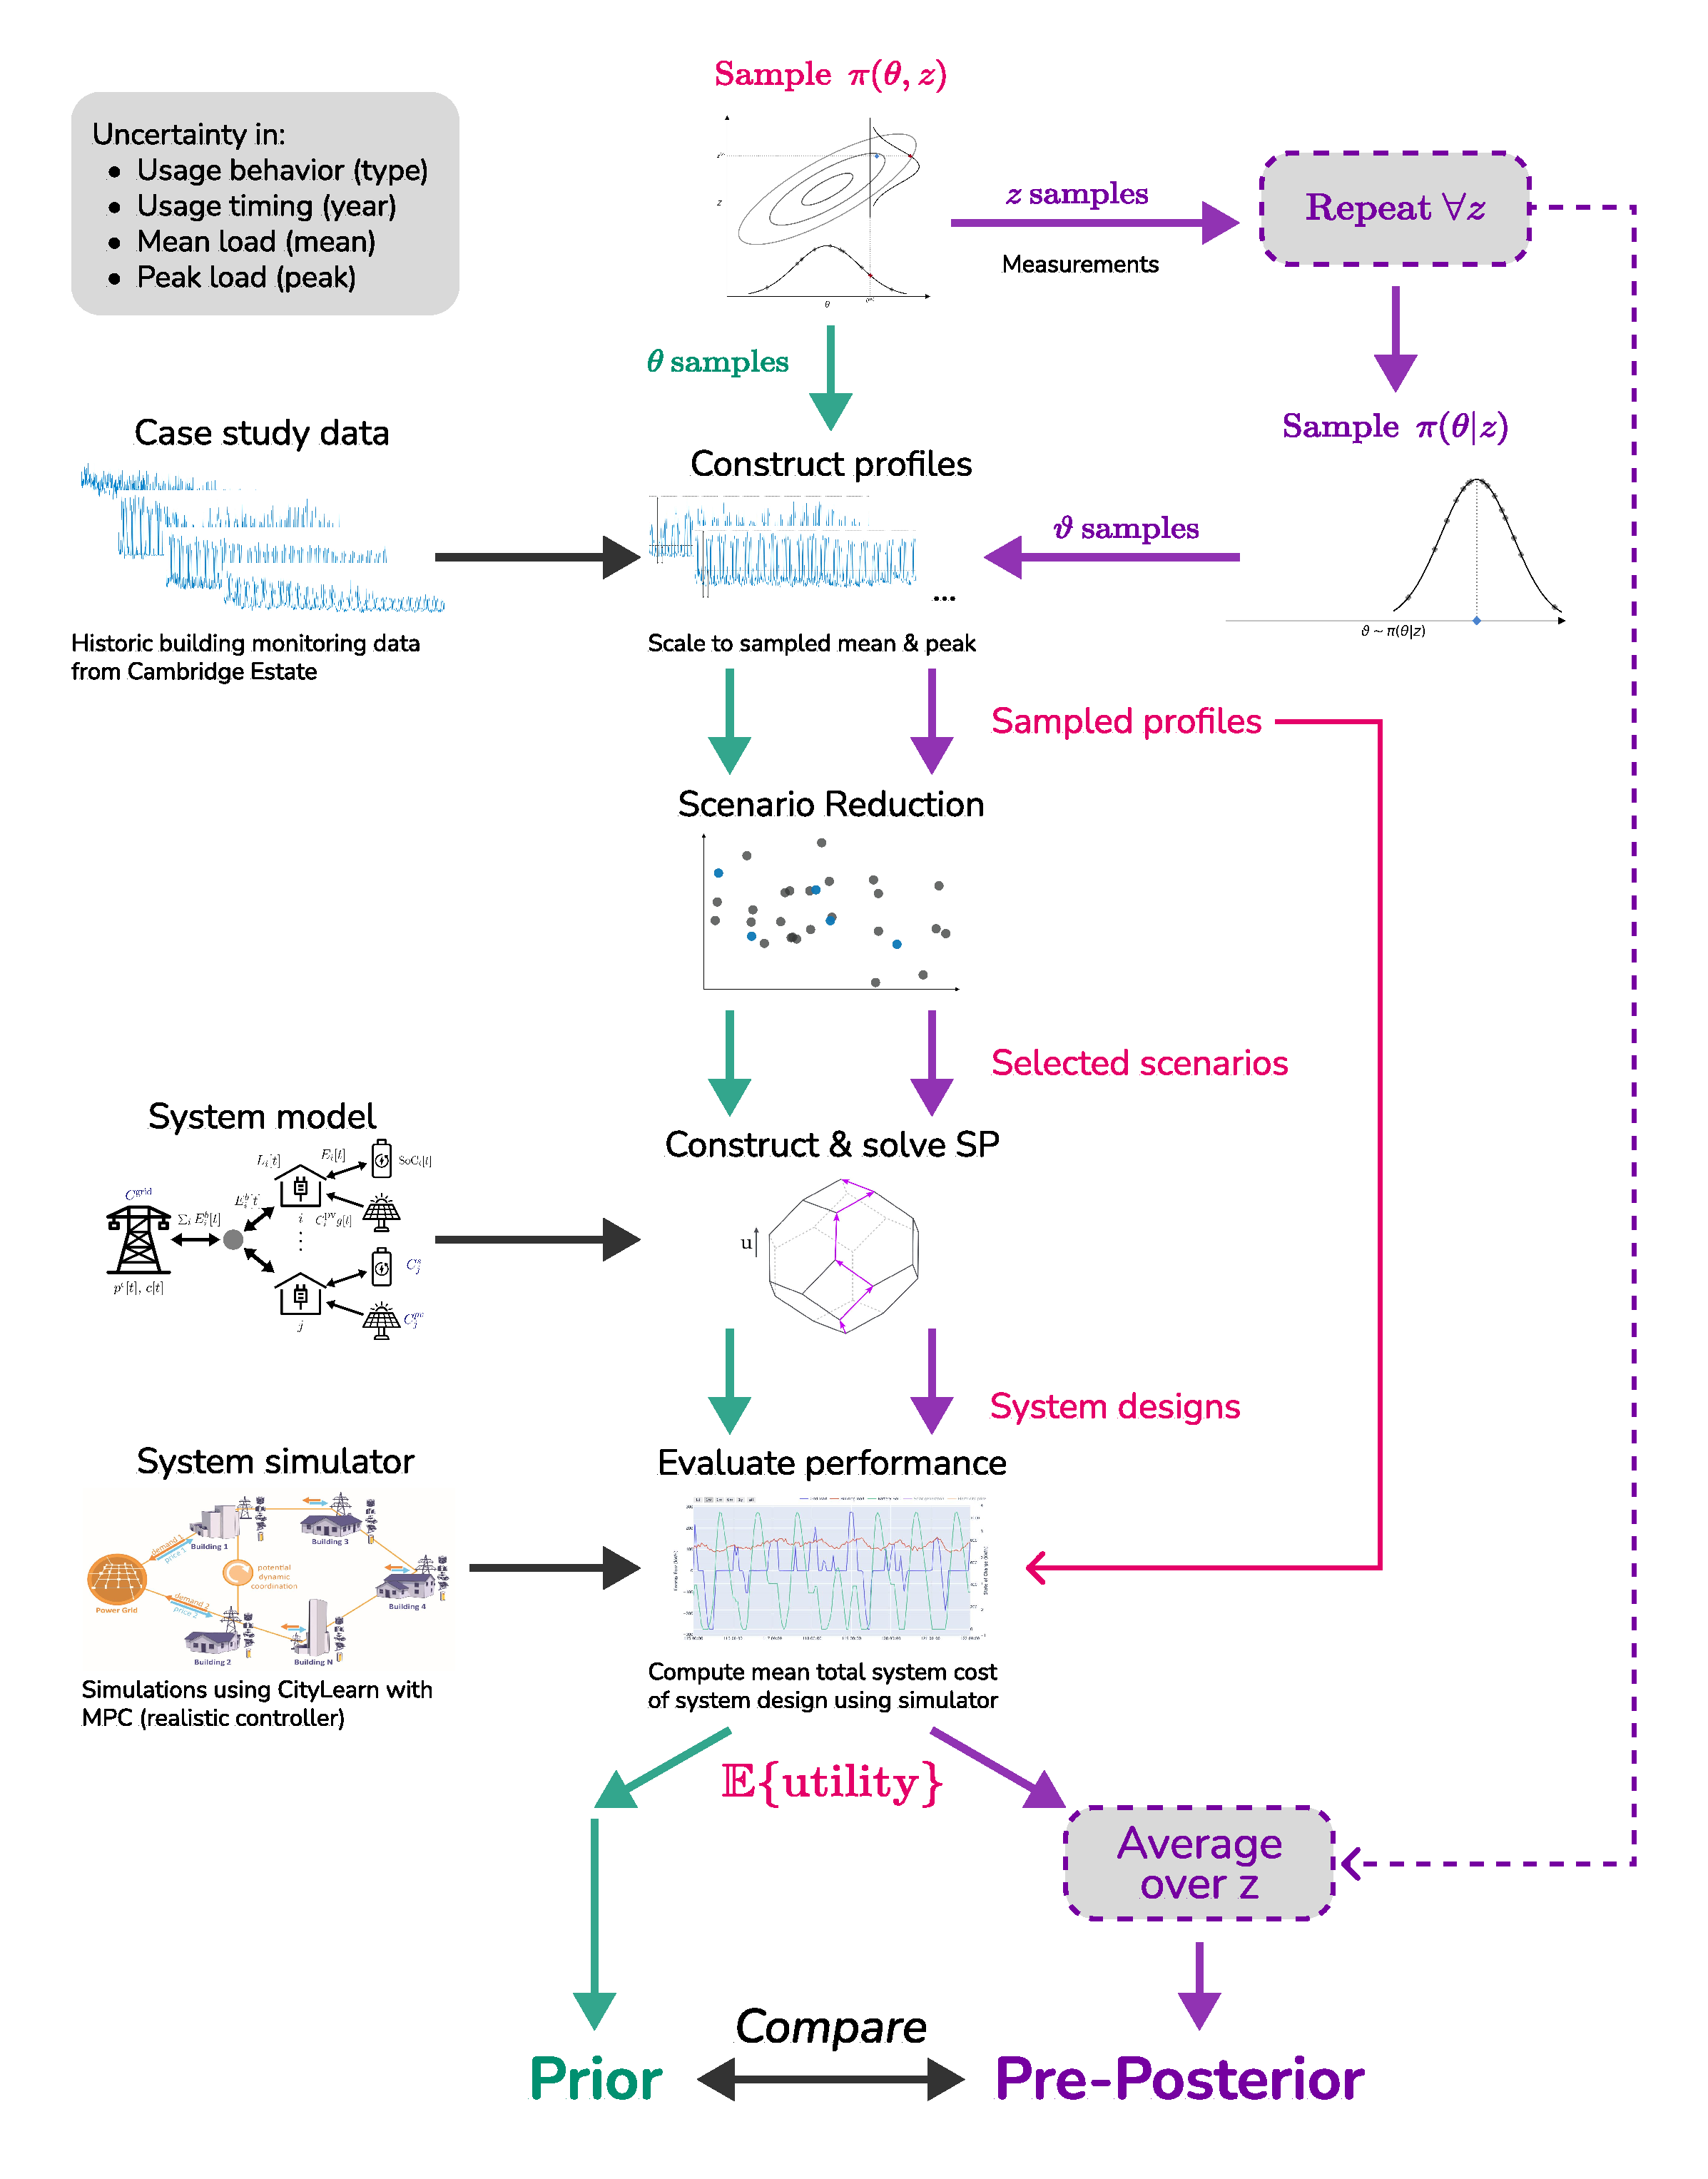
\includegraphics[width=\linewidth]{districts_methdology.pdf}
    \caption{Methodology for computing \glsxtrshort{voi} for case study district energy system design task.}
    \label{fig:districts-method}
\end{figure}


\newpage
%********************************** Results section **************************************
\section{Results \& Discussion} \label{sec:districts-results}

\subsection{System design without load monitoring} \label{sec:districts-prior-design}

%%! Think about narrative (VoI, load monitoring). What is relevant to discuss here?

%% !Briefly! explain and present initial (prior) design
% Discuss cost reduction provided by installing solar battery system - compare to costs without, with only solar, with only battery - *actually* is this part of the story? maybe just briefly mention the % cost reduction provided by the solar-battery system (and maybe specifically carbon emissions contribution also)
% No grid capacity exceedance (in 1000 samples) - design & controller about to manage system properly (important for context, we can have confidence in requested grid capacity) - grid impact can be limited to known/contracted value in all(?) cases

% Discuss impact of uncertainties on simulation outcomes for prior design - show that they are signficant, demonstrate that there is variation due to load profiles (uncertainty), and discuss contributions (mean most influential, shape signficant, peak uncorrelated)
% There is significant variability in cost outcomes due to load uncertainties which *could* be addressed/reduce high costs through measurement

A district containing 5 university buildings, without constraints on asset sizing, is considered as a base case. Initially the case where no building load monitoring is used is considered. Load profile scenarios were sampled from the prior distribution, which represents the behaviour of a generic university building, and the Stochastic Program model described in \Cref{sec:districts-SP} was used to size the solar-battery systems and grid connection capacity using these prior scenarios.

The optimized (prior) design installs 4,910 kWh of batteries and 2,790 kWp of solar panels across the 5 buildings, roughly evenly distributed, and contracts 1,230 kW of grid connection capacity (2.5 times the mean electrical load of the district of 500 kW). From operational simulations, the average lifetime cost for the system (the prior expected utility) was determined to be £22.432m over a 20 year operational lifetime, or £1.122m/year. Comparing to the case where no solar-battery systems are installed in the buildings, which results in a mean operational cost of £1.839m/year, this investment in local generation and storage reduces total operating costs for the energy system by 39\%. Additionally, the embodied carbon emissions of providing energy are reduced by 64\%, and the required grid connection capacity is reduced by 27\%. Further, the practical building controller did not exceed the contracted grid capacity in any of the 256 sampled scenarios simulated. These results validate the ability of solar-battery systems to simultaneously reduce the overall cost of energy provision, embodied carbon emissions, and the grid impact of the district. Further details of the optimized system design and its performance across the simulated scenarios are provided in \ref{app:districts-prior-design}.

Fig. \ref{fig:districts-prior-costs} plots the distributions of simulated system costs and corresponding Levelized Costs of Energy (LCOEs) when the prior design is operated for each sampled load scenario. It shows that the uncertainty in building load causes significant uncertainty in the total operating cost of the system. As the LCOE normalizes the operating cost by the total energy usage of the buildings, it removes the contribution of mean load to cost variability. The standard deviation of the LCOE distribution is 3.8\%, compared to 10.2\% for the total cost distribution, comparing Fig. \ref{fig:districts-prior-costs-lcoe} to Fig. \ref{fig:districts-prior-costs-total}. This demonstrates that mean load is the greatest driver of cost variability, but that the remaining uncertainties (peak load and load profile shape) also make a significant contribution.
There is found to be no correlation between the peak electrical load of the district and the total operating cost across all scenarios, indicating that peak load has little to no influence on the cost of operation. This can be justified as the sizing of the battery units to perform bulk energy arbitrage results in them having a power capacity of 1,960 kW, meaning they can handle the highest possible peak load of the district of 2000 kW (of which only 770 kW needs to be shaved to avoid exceeding the grid connection capacity). As a result, in almost all simulated scenarios no grid excess charges are incurred. Though the peak may occur when electricity is expensive, as they are infrequent there is only a small impact on the overall electricity cost. The operational behaviour of the district energy system and the factors influencing system design are discussed further in \ref{app:districts-prior-design}.

\begin{figure}
    \centering
    \subfloat[Total system costs.]{
        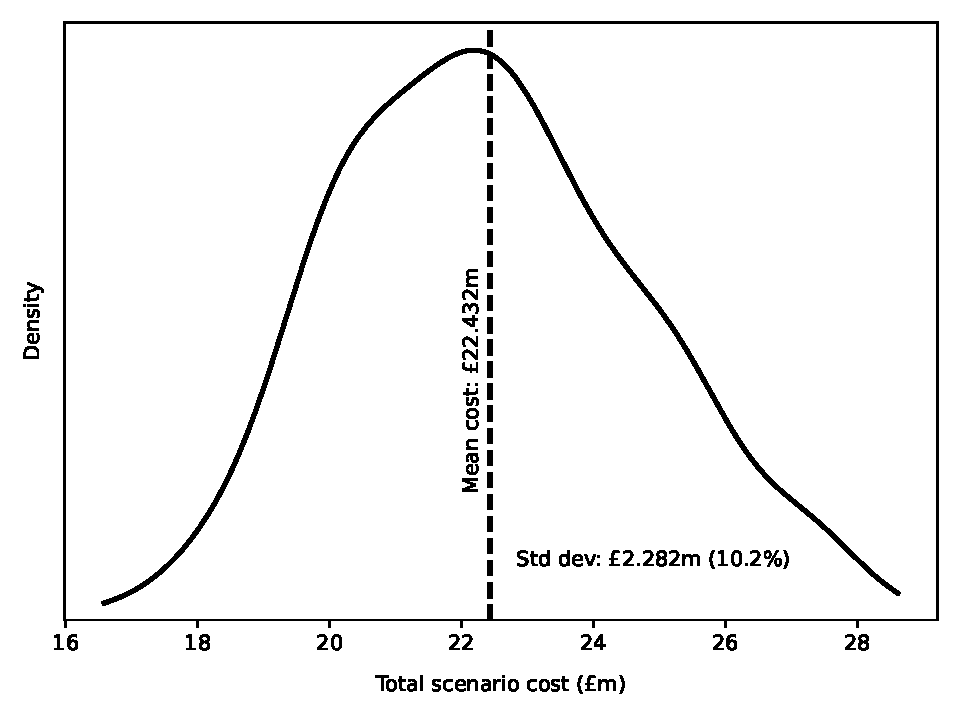
\includegraphics[width=0.475\linewidth]{districts_prior_total_costs.pdf} \label{fig:districts-prior-costs-total}
    }%
    \hfill
    \subfloat[LCOEs.]{
        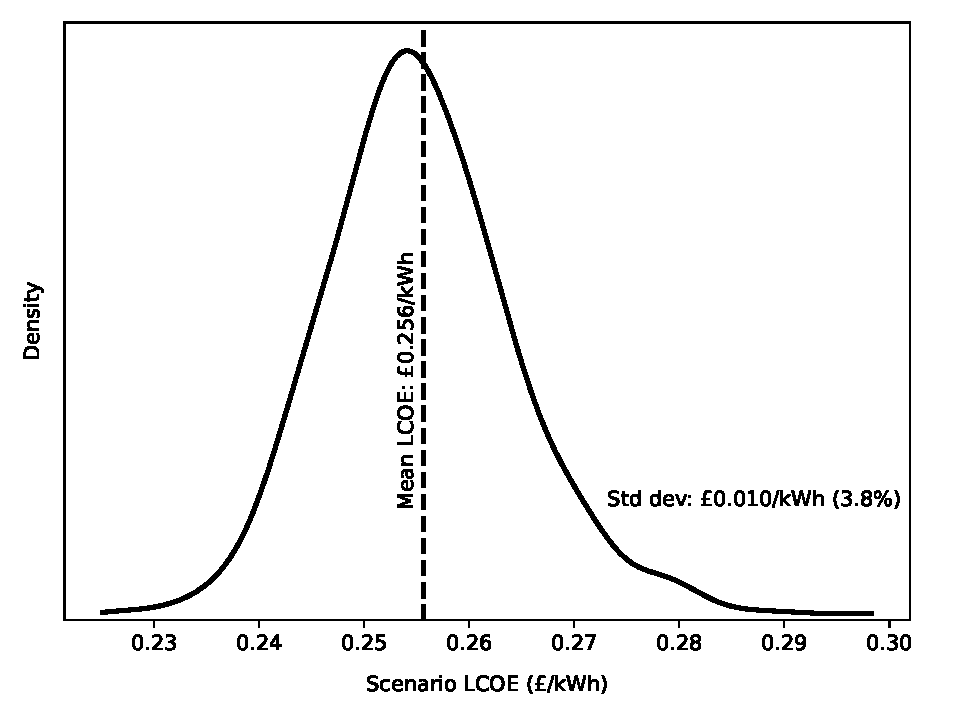
\includegraphics[width=0.475\linewidth]{districts_prior_lcoes.pdf} \label{fig:districts-prior-costs-lcoe}
    }
    \vspace*{-0.2cm}
    \caption{Distribution of simulated total system costs and LCOEs for prior system design over sampled building load scenarios.} \label{fig:districts-prior-costs}
\end{figure}

This analysis demonstrates that uncertainty in mean electrical load of the district is the largest driver of operational cost uncertainty, responsible for over half of induced variability, but that the other uncertainties (in peak load, load profile shape, and solar generation) also have a significant influence on cost.
% Add interpretation comment? E.g. "This is because ..."
Therefore there might exist scope to reduce the total system cost by reducing uncertainty in these factors, and tailoring the system design to the energy usage behaviour of the true target building\footnote{This tailoring of the system (improved design) could reduce not only the highest cost scenarios for the prior case (the right tail of Fig. \ref{fig:districts-prior-costs-total}), but also costs in the scenarios which are already cheap, as the system design does not need to compromise to keep costs down in the expensive cases, hence less generation and storage capacity can be used, reducing asset costs.}.
% So VoI study is meaningful (bit more nuance, but good enough)
% Explicitly state existing methods stop here and discuss weakness of conclusion provided
Most existing analyses, such as those in \citep{mavromatidis2018ReviewUncertaintyCharacterisation,prataviera2022EvaluationImpactInput}, or other purely statistical approaches \citep{pang2020RoleSensitivityAnalysis}, stop at this stage and put forward the conclusion that reducing uncertainty in the model's inputs (here, building load) would significantly reduce uncertainty in the model output (the operating cost of the system). However, this outcome does not provide any indication about whether this uncertainty reduction would affect the decision made, and so cannot quantify its importance for supporting decision making.


\subsection{Value of building load monitoring} \label{sec:districts-voi-results}

%% Overall
% Scatter plot prior and posterior designs on axes of total battery and pv capacities, with grid cap as colour
% Plot distributions of prior and posteriors costs?
% Might also be interesting to look at things like average grid cap for posterior solns
% Pick out average carbon emissions savings - interesting point is even if measurement only breaks even may still want to do it for the carbon

% Discuss interpretation and importance of VoI result - value is significant, but not huge

The On-Policy \glsxtrshort{voi} framework presented in \Cref{sec:methodology-on-policy-voi} was used to quantify the economic benefit of uncertainty reduction from building load monitoring to support the design decision of sizing solar-battery systems and grid connection capacity for the district. A set of 256 hypothetical monitoring measurements were sampled using the probability models defined in \Cref{sec:districts-prob}, and the procedure of using Stochastic Programming to design (size) the system, and simulations to evaluate its performance, was repeated for each hypothesised measurement using samples drawn from the corresponding posterior distribution. This process considers the following questions;\\

\begin{cbox}[colback=Aquamarine!10!white]{}
    Were the building monitoring systems to have returned a given measurement, reducing uncertainty in the building load profiles: What would the optimal district energy system design be? And what would be its average operational cost under the remaining load uncertainty?
\end{cbox}\

Fig. \ref{fig:districts-posterior-designs} plots the total asset capacities of the optimized system design for each hypothesised load monitoring measurement (the posterior designs, each indicated with a circle), and compares them to the prior system design (indicated by a diamond).
It shows that the optimal asset sizes vary significantly with the load monitoring measurements, which provide information about the true energy usage behaviour of the district buildings, by approximately $\pm$20\% for each of solar, battery, and grid total capacities. These posterior optimal asset capacities are strongly correlated with the mean load of the posterior distribution, see Fig. \ref{fig:districts-posterior-designs-correlation}.
% Comment on linear trends and relative spreads about these? (In appendix? Def. for thesis, discuss causality)

\begin{figure}
    \centering
    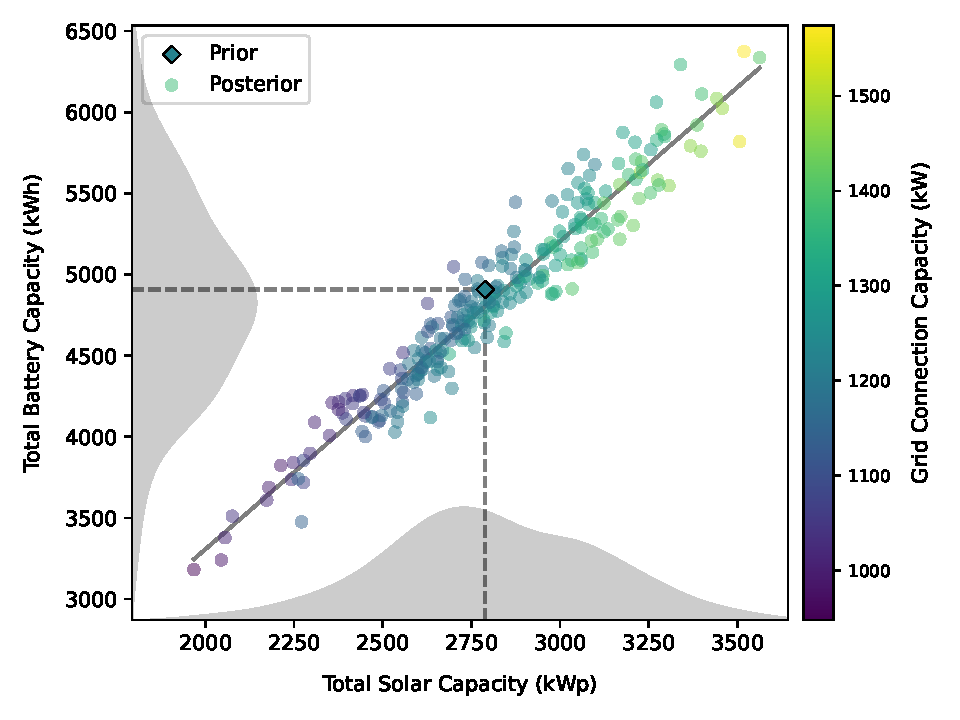
\includegraphics[width=0.8\linewidth]{districts_unconstr_5b_posterior_designs.pdf}
    \caption{Total asset capacities in optimized system designs for each hypothesised load monitoring measurement. \textit{Prior system design indicated with diamond.}}
    \label{fig:districts-posterior-designs}
\end{figure}

\begin{figure}
    \centering
        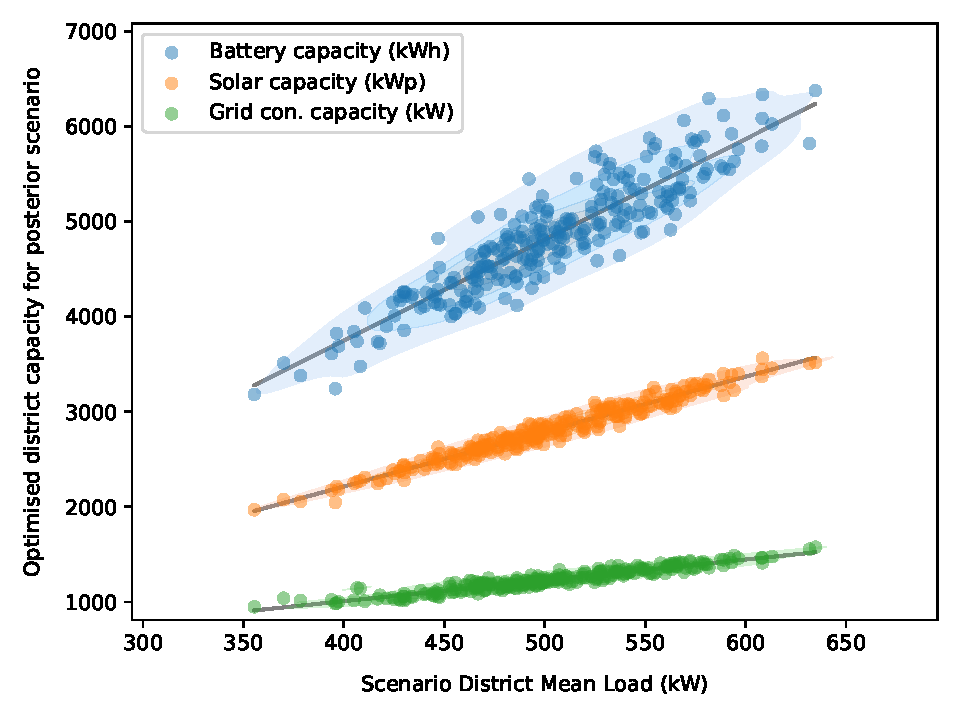
\includegraphics[width=0.8\linewidth]{districts_unconstr_5b_posterior_designs_correlation.pdf}
        \caption{Correlation between total asset capacities in posterior designs and mean load over posterior sampled building load scenarios used for design (from scenario reduction).}
    \label{fig:districts-posterior-designs-correlation}
\end{figure}

A sensitivity analysis studying the influence of input uncertainties on the optimal system design, such as those performed in \citep{mavromatidis2018UncertaintyGlobalSensitivity} \& \citep{pickering2019DistrictEnergySystem}, would stop at this point and conclude that the uncertainty reduction from building monitoring has a substantial impact on the optimal system design, and is therefore important information to gather for achieving a design close to the optimal for the district as built. However, this approach fails to address the actual goal of decision making. From the perspective of the decision-maker, they are not concerned with what decision is taken, but instead with how well on average that decision performs, i.e. its expected benefit/utility. Rather than the difference between the posterior designs and prior design themselves, the metric that is important for determining whether the building monitoring information is valuable for supporting decision making is the difference between their \textit{performance}. I.e. how much lower the lifetime cost of the district energy system is on average as a result of performing the system design with the building monitoring information, and the resulting reduced uncertainty. This metric is called the \glsxtrlong{voi} (\glsxtrshort{voi}), defined in \Cref{sec:methodology-voi}.

Figures \ref{fig:districts-posterior-costs} \& \ref{fig:districts-posterior-lcoes} plot the distributions of total system costs and LCOEs achieved by the prior and posterior designs across the simulated building load scenario samples. The average lifetime cost for the posterior designs (the pre-posterior expected utility) is found to be £22.147m over the 20 year lifetime (£1.107m/year). Comparing to the prior expected utility of £22.432m, the \glsxtrlong{voi} for building load monitoring is estimated at £284k, or 1.27\% of the prior cost.

This \glsxtrshort{voi} result demonstrates that using building monitoring to support energy system design for this district reduces the average total cost of the energy system by under 1.5\%. This methodology leads to a conclusion that is very different from those provided by existing analyses, which suggest that the uncertainty reduction would have a large impact on the design task. Further, the insights provided by \glsxtrshort{voi} are far more aligned with the goals of the decision maker.\\
% To add - whilst optimal designs vary significantly from prior, their performance does not

\begin{figure}[h]
    \centering
    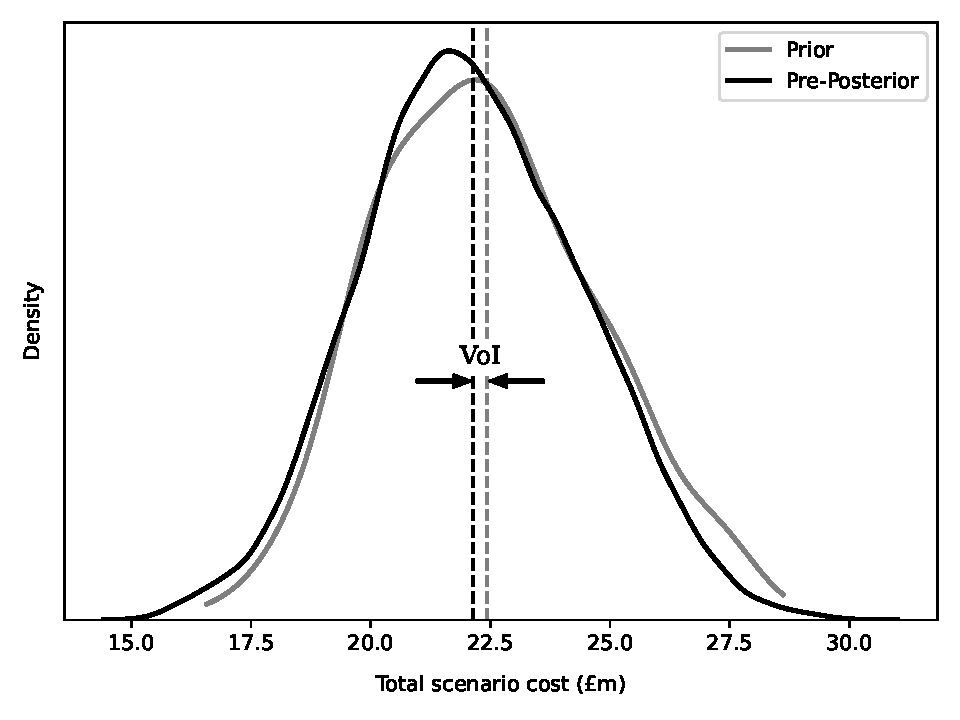
\includegraphics[width=0.75\linewidth]{districts_unconstr_5b_posterior_total_costs.pdf}
    \caption{Comparison of simulated total system cost distributions for prior and pre-posterior cases.}
    \label{fig:districts-posterior-costs}
\end{figure}

\begin{figure}[h]
    \centering
    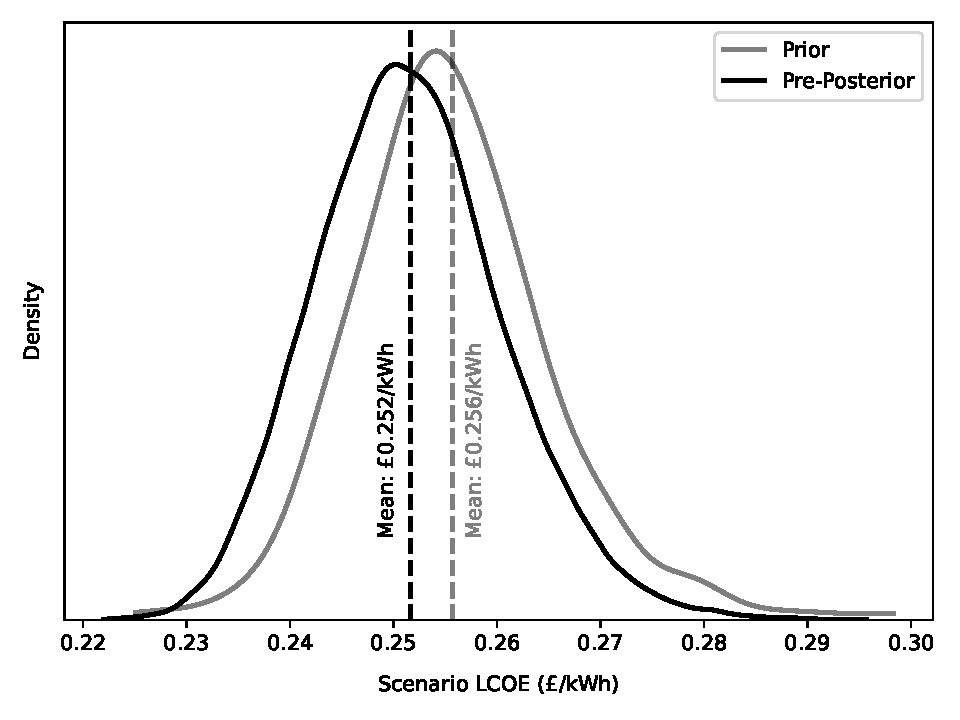
\includegraphics[width=0.75\linewidth]{districts_unconstr_5b_posterior_lcoes.pdf}
    \caption{Comparison of simulated LCOE distributions for prior and pre-posterior cases.}
    \label{fig:districts-posterior-lcoes}
\end{figure}

\newpage
Gathering building monitoring data to improve the sizing of the solar-battery systems would only be worthwhile if the cost of collecting that data is less than the \glsxtrshort{voi} value computed.
Installing the solar-battery systems was found in Sec. \ref{sec:districts-prior-design} to reduce operational costs by on average £717k/year. Therefore, by itself the option cost of delaying installation of the solar-battery systems for one year to monitor the buildings and install an optimized system outweighs the benefits of that design optimization (provided by the uncertainty reduction from measurement). The actual cost of performing building monitoring would be higher due to costs associated with delaying the construction project. Hence, the \glsxtrshort{voi} analysis shows that, for this particular energy system design task, reducing uncertainty in the building load profiles through monitoring is not economically worthwhile. I.e. the benefit it provides to improving decision making is less than its cost.
% Add more discussion of interpretation and pratical importance? Or leave for \ref{sec:districts-practical-importance}?

\newpage
\subsubsection{Relative importance of reduced uncertainties} \label{sec:districts-contributions}

% Show results for VoI for partial information from each parameter separately and compare to overall
% Mean variation accounts for all of total VoI! This is important because this wouldn't be picked up by traditional experimental design (would suggest profile variance reduction), so is a value add from VoI (meaningful insight only it can provide)

The relative importance of each aspect of building load uncertainty (\texttt{type}, \texttt{peak}, \texttt{mean}) for supporting decision making was investigated by repeating the \glsxtrshort{voi} analysis for uncertainty reduction in each parameter independently. Table \ref{tab:districts-VOI-contributions} presents the results of this analysis. Similarly to the classical sensitivity analysis performed in \Cref{sec:districts-prior-design}, reducing the uncertainty in mean load is found to be of greater importance than uncertainty in the profile shape and peak load, providing roughly half the available benefit to decision making.\\
%However, the VoI based importance analysis provides two key insights which could not be identified by purely statistical analysis.

\begin{table}[h] % For thesis: add design figure for each case and discuss differences
    \centering
    \renewcommand{\arraystretch}{1.1}
    \begin{tabular}{c|c|c} \toprule \toprule
        Reduced uncertainties & Expected total cost (£m) [\%] & \glsxtrshort{voi} (£k) [\%] \\ \midrule
        None (prior) & 22.432 [100.0\%] & -- \\
        \texttt{type} & 22.573\, [100.6\%] & 0\textsuperscript{\textdagger}\, [0.0\%] \\
        \texttt{peak} & 22.401\, [99.87\%] & 30\,\:\, [0.14\%] \\
        \texttt{mean} & 22.276\, [99.31\%] & 156\, [0.69\%] \\
        All & 22.147\, [98.73\%] & 284\, [1.27\%] \\
        \bottomrule \bottomrule
    \end{tabular}
    \smallskip
    \caption{Expected system operating cost and \glsxtrshort{voi} for separate uncertainty reduction in load parameters.}
    \label{tab:districts-VOI-contributions}
\end{table}

\customfootnotetext{\textdagger}{This value is actually estimated to be -£141k (-0.63\%), but is clipped to 0 as \glsxtrshort{voi} values are defined to be non-negative. This highlights the numerical error in the \glsxtrshort{voi} calculations. However, even plus/minus this level of error, the \glsxtrshort{voi} values are still small relative to the cost of measurement, and the conclusions remain valid.}

While uncertainty in the peak load and load profile shape of the buildings is responsible for a significant portion of the overall cost variability, collecting information which reduces uncertainty in only one of these parameters provides very little improvement for solar-battery system design. In fact, reducing uncertainty in the \texttt{type} parameter, which corresponds to obtaining a probabilistic model of the patterns and timing of energy use specific to each building, does not improve the designs at all. So, by itself, performing detailed occupancy modelling to generate precise time-of-use energy profiles for the buildings would not be helpful for supporting the design of this district energy system.

However, when all three uncertainties are reduced simultaneously, the \glsxtrshort{voi} is significantly greater than the sum of the separate contributions\footnotemark. Therefore, if more precise information is available about the mean load of the buildings, then information about the peak load and load profile shape can be used to further improve the design. This result demonstrates that designers must consider not only whether they have the correct information to support their decision making, but the correct combination of information to unlock maximum value. Insights of this kind can only be obtained by applying the \glsxtrshort{voi} methodology.

\footnotetext{This is possible as the \glsxtrshort{voi} is not additive. Different measurements can either contain complementary information which is more useful for decision making when combined, or conversely can contain the same information, meaning the combination of measurements provides less total benefit \citep{difrancesco2023SystemEffectsIdentifying}.}


\subsubsection{Alternative system scenarios} \label{sec:districts-alt-systems}

% Discuss practical constraints on solar and show VoI is zero: decision devolves as battery set by solar (used for improving self-consumption mostly) and so when solar is known (i.e. best to be max) then there is little decision left to make on the battery
% Discuss setup with only 1 building: VoI higher as the relative variance in overall (district) mean load is higher (due to lack of CLT effect), discuss relevance for designing larger systems (the more buildings in scope the less useful info as mean values are most consistent - lower variance)

The same energy system sizing task was investigated in two alternative building system scenarios to study how the \glsxtrshort{voi} of building load monitoring varied, and whether the conclusions regarding its economic usefulness changed from the base case. These two cases involve designing for a single building energy system, and designing for a district with constrained solar capacity.

Often adjacent buildings are owned by independent parties, and their energy systems are installed at different times with limited cooperation. So, solar-battery systems are frequently designed independently for each building, and for large consumers (e.g. industrial sites) each must contract their own grid connection capacity. Repeating the \glsxtrshort{voi} analysis with a single building, i.e. without district effects, the \glsxtrshort{voi} was found to be £99k, or 2.17\% of the prior cost of £4.568m. Whilst in this case the \glsxtrshort{voi} has increased relative to the prior cost, it is still lower than the annual benefit of installing the solar-battery system, which is £145k/year. Therefore, it is still not economical to perform building monitoring to support design. It is proposed that the reduction in proportional \glsxtrshort{voi} as more buildings are included in the district is caused by the variability (standard deviation) of the district mean load. Reducing uncertainty in mean load was found to be the most influential factor for improving system design in \Cref{sec:districts-contributions}, and the district mean load was the greatest driver of cost uncertainty, see \cref{sec:districts-prior-design}. As mean load distributions are taken to be independent for each building, by the Central Limit Theorem, the standard deviation of the district mean load as a fraction of that load decays with the number of buildings in the district as $1/\sqrt{n}$. Therefore, measurement of the buildings provides less information on the district mean load the more buildings there are. Hence, the less valuable that information is for supporting design. This implies the more buildings there are in the district, the better decisions regarding total storage capacity for bulk energy arbitrage average out across the district, and the less sensitive they are to uncertainty in the mean load.

In many European countries, due to land constraints, buildings are built tall to accommodate more floor area, and do not have spare open spaces nearby. This limits their available roof area, and so the quantity of local solar generation they can accommodate to decarbonize their energy usage. The \glsxtrshort{voi} analysis was repeated for a district of 5 buildings with a constraint on the maximum solar capacity (kWp) per building. This constraint was derived using roof area data from the Cambridge dataset \citep{langtry2024CambridgeUniversityEstates}. University buildings in Cambridge with around 100 kW mean load ($\pm$20\%) were found to have a roof area of approximately 1000 m$^2$. Assuming a solar panel power density of 0.15 kWp/m$^2$ \citep{gawley2022InvestigatingSuitabilityGIS,gagnon2018EstimatingRooftopSolar}, leads to an optimistic constraint of 150 kWp of solar capacity per building. With this constraint, the \glsxtrshort{voi} of building load monitoring was found to be only £13k, or 0.05\% of the prior cost of £29.075m. Under the formulated operational objective, the primary benefit of the battery system is derived from arbitraging the cheap, zero-carbon solar energy generated by the building solar PV. This is why in the base case, the installed battery capacity of the optimal designs scale linearly with the solar capacity, see Fig. \ref{fig:districts-posterior-designs}. For all scenarios in the solar constrained case, the maximum quantity of solar PV is installed, and so the value that can be derived from arbitraging that energy is fixed. Whilst the optimized system designs for each hypothesised measurement in the constrained case show some variability in the battery and grid capacities installed, these additional capacities provide only small additional benefit from arbitraging cheap and/or low carbon grid electricity, and these benefits are not much more than their costs. As a result, updating the system designs (battery sizings) with improved information provides very little benefit in this case.\\


\subsection{Planning risk reduction}

% Discuss standard deviation & range of outcomes pre and post measurement (highlight reduction) and discuss importance for project planning, even if there is little influence on mean cost; caveat of VoI framework is assumption of risk neutrality, which energy system designers certainly are not

In the \glsxtrshort{voi} framework, decision makers are assumed to be risk neutral, and the benefit of data collection is quantified in terms of how much it is able to improve the \textit{average} performance/utility of decisions made. However, in the energy field, decision makers are sensitive to risk, as it affects their ability to raise capital as well as the interest rates they can access, which impacts the cost of energy decarbonization and so their ability to afford it.
For the prior optimal design in the base case, the range of system lifetime costs over the simulations was found to be £16.580m to £28.616m, from a mean of £22.432m (see Fig. \ref{fig:districts-prior-costs-total} in \Cref{sec:districts-prior-design}). This 54\% cost range could be problematic for the financial planning of the district energy system, particularly as the operational costs of energy system (electricity, carbon, and grid excess costs) vary from £6.360m to £18.396m.

The information provided by load monitoring can be used to support this financial planning, as it reduces uncertainty in the operational cost of energy system. In the experiments, after a hypothetical monitoring measurement was taken, the system design was optimized for the corresponding posterior load distribution, and the operation of this system was simulated for scenarios sampled from that posterior, leading to a distribution of total system costs for the design. Fig. \ref{fig:districts-posterior-variability} plots the distributions over the hypothesised measurements of the standard deviations and ranges of the simulated total system costs for each design (corresponding to a hypothesised measurement), as a proportion of the value for the total cost distribution for the prior design (shown in Fig. \ref{fig:districts-prior-costs-total}). The standard deviation and range of the costs are significantly reduced after measurement, demonstrating that whilst designing the energy system with load monitoring information does not significantly reduce the average system cost, at the time of design and so financing, it substantially reduces the uncertainty in what the system cost will be. Therefore, there may be some additional value to this information for supporting financial decision making. This motivates the use of \glsxtrshort{voi} to study the benefit of data collection to support risk averse decision making, which has yet to be done in an engineering context. This would require the expansion of utility/objective functions to account for the cost of risk. Existing studies have incorporated risk measures into district energy system design objectives to account for risk aversion \citep{pickering2019PracticalOptimisationDistrict}, and these methods are applicable to studying \glsxtrshort{voi}.\\

\begin{figure}[t]
    \centering
    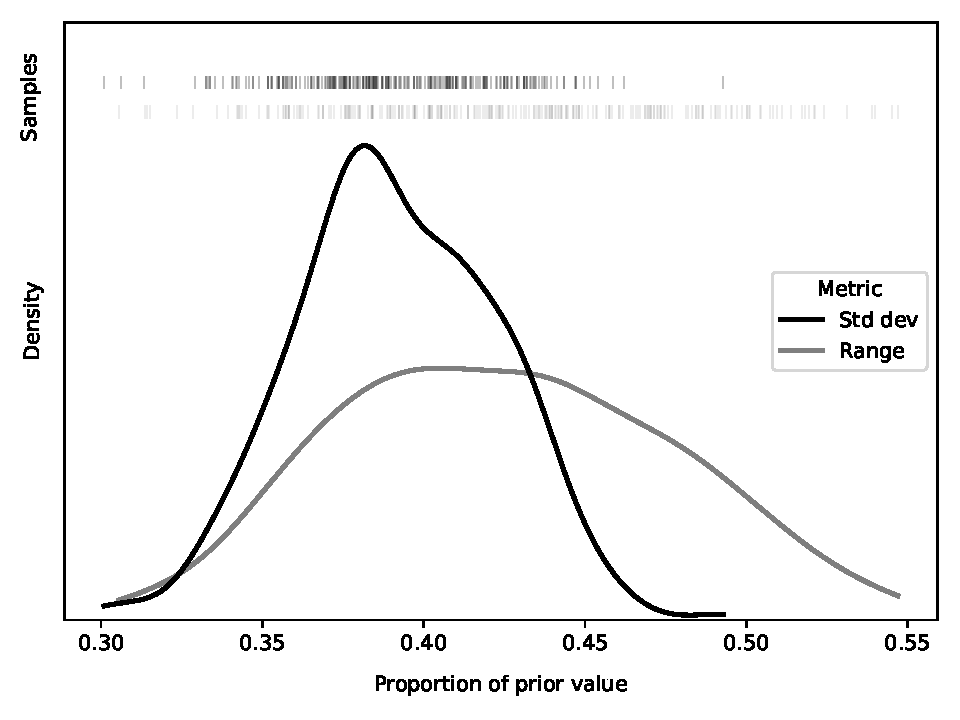
\includegraphics[width=0.75\linewidth]{districts_posterior_cost_variability.pdf}
    \caption{Distribution over hypothesised measurements of standard deviation and range of total cost distribution of optimized system design for each hypothesised measurement (simulated for scenarios drawn from corresponding posterior distribution).}
    \label{fig:districts-posterior-variability}
\end{figure}


%\newpage
\subsection{Practical importance \& limitations of study} \label{sec:districts-practical-importance}

% Discuss interpretation and justification (reseaons for) of results and importance for practitioners - see online notes about discussion points
% An important implication of this work is the effort that should be expended by energy system models in refining their load profiles used for design. These results suggest that using population level priors leads to very similar designs, and leaves little value on the table (2% for a small district), so suggests that these priors are sufficient - provides first evidence of sufficiency of current standard practice
% Its really worth spending time and effort finding out mean load (e.g. detailed room modelling \& communication between designer and occupants) - in fact all decision making benefit comes from this; but not so much for profile shape (this has important implications for best practice around example profiles for building design - a good guess is good enough); so modelling of mean load critical, meaning communication between building developer and building occupier(s) is very valuable during design phase (e.g. perform detailed room by room building usage modelling)

% Solar generation dominates design problem because it is so cheap c.f. grid electricity, and much more peaky than load
% So uncertainty in solar generation very important, not considered in this study, but also there's a limited amount that can be done to reduce it through measurement (i.e. existing data, e.g. RenewablesNinja like models, provide very strong prior)
% Also other uncertainties not considered - in this case done for clarity, but still, would be important further work

% Usual caveats that VoI values are not predictable problem to problem, so study of wider problems required, both uncertainties and problem setups

The \glsxtrlong{voi} calculations performed in this study (\Cref{sec:districts-voi-results}) demonstrate that, for the district energy system design task considered, hourly building load data is not worth collecting to support design, i.e. its benefit is less than its cost. This allows practitioners to avoid wasting time and resources on monitoring, and confirms that an opportunity for reducing the cost of decarbonizing building energy is not being missed. Further, showing that limited value is derived from reducing building load profile uncertainty indicates that population level priors constructed from monitoring data from existing buildings are sufficient for designing energy systems in unseen buildings. This provides the first numerical evidence to suggest that current industry practice of designing energy systems using standard building profiles achieves near optimal design performance. However, it is strongly recommended that using Stochastic Optimization techniques which seek designs that perform well over the distribution of building behaviours is critical.

\Cref{sec:districts-contributions} found that reducing uncertainty in only the mean load provided most of the available decision support benefit. This result is highly pertinent for the design of both new building energy systems, and energy retrofits of existing buildings. For new buildings, while in this case study load monitoring is not worthwhile to support design, the reduction in mean load uncertainty does still provide significant benefit. Therefore, effort should be directed to producing an accurate statistical estimate of building mean load, for instance through detailed building usage modelling, i.e. at room level. Communication between the energy system designer and building owners/occupants regarding the intended use of the building is critical to enabling accurate load estimates, and so low cost energy system designs. For the case of building retrofits, monthly gas and electricity metering data are available. This enables a very good estimate of the mean building electrical load after retrofit, and so using hourly metering data for system sizing would provide little additional benefit.

In this study, uncertainty in building load and solar generation only were considered for the sake of clarity when demonstrating the \glsxtrshort{voi} methodology. However, several other important factors in the district energy system are subject to significant uncertainty, such as electricity prices (which are determined by the future grid generation mix and weather conditions), asset operational lifetimes which impact their effective cost, and battery degradation (neglected in this model) which affects the efficiency and capacity of the battery units over their lifetime. More detailed system design work should consider these uncertainties in the Stochastic Optimization model to include their influence on the design task and resulting cost distributions. A key difference with these uncertainties is that they are not practically measurable at the time of design, and so should not be studied using \glsxtrshort{voi}, as the resulting values would not be meaningful.

Performing \glsxtrshort{voi} calculations is highly computationally intensive. In the On-Policy \glsxtrshort{voi} framework, system designs must be both determined and evaluated for a large number of hypothesised measurements to achieve sufficient statistical accuracy in the mean utility estimates to enable the correct identification of the true \glsxtrshort{voi} value over statistical error. This limits the complexity/resolution of building energy system models that can be studied with the framework. However this computational cost is minimal compared to the potential cost savings of avoiding project delays to gather unnecessary building monitoring data. The computational requirements of the \glsxtrshort{voi} calculations from this study are discussed further in \ref{app:districts-numerics}.

Finally, the key critique of the \glsxtrshort{voi} framework is that \glsxtrshort{voi} values computed are only valid under the particular model formulation studied, including its assumptions \citep{langtry2024RationalisingDataCollection}. \glsxtrshort{voi} results cannot be generalized, and changes in the problem setup can significantly alter the \glsxtrshort{voi}, as seen when introducing solar capacity constraints in \Cref{sec:districts-alt-systems}. Therefore, further investigation of \glsxtrshort{voi} for supporting building energy system design is required to confirm whether the conclusions made in this study are consistent across different building energy systems (e.g. those in different climates or with different energy usage patterns), design objectives, and modelling assumptions. The \glsxtrshort{voi} methodology should also be used to investigate the importance of reducing other uncertainties in buildings (such as thermal properties of the envelope), and whether performing other types of measurements could provide significant improvements for the design of energy systems.\\


%********************************** Conclusions **************************************
\section{Conclusions} \label{sec:districts-conclusions}

This chapter investigated the economic benefit of gathering hourly building energy usage data to support the design of a district energy system, specifically involving the sizing of distributed solar-battery systems to decarbonise building energy usage under grid constraints. A case study district energy system containing 5 university buildings was considered, with probabilistic models of the building load profiles constructed using historic electricity metering data from the Cambridge University estate.

The uncertainty in building load was found to have a significant impact on the operating cost of the system, causing a $\pm$30\% variation in total cost for the energy system designed without monitoring data available. Also, reducing uncertainty in the building load by collecting monitoring data had a significant effect on the optimized energy system design, with total installed capacities of solar, battery, and grid connection varying by roughly $\pm$20\% across the hypothesised measurement values. Therefore, existing methods which stop at either of these two points would conclude that collecting hourly metering data would have a significant effect on system design.

However, performing a \glsxtrlong{voi} analysis using the On-Policy \glsxtrshort{voi} framework demonstrated that reducing load uncertainty via monitoring would reduce the overall energy system cost by less than 1.5\% on average through improved design. This was found to be less than the cost savings achieved by installing solar-battery systems to reduce operating costs over the period needed to monitor the buildings and install systems with improved design. Therefore, collecting hourly building monitoring data was determined to be not economically worthwhile for supporting the design of the studied district energy system.
Reducing uncertainty in only the mean load was found to provide most of the available decision support benefit. This means that for building retrofits where the mean building load can be well estimated from historic monthly energy usage data, using hourly metering data would provide little additional benefit for system design.
So while \Cref{chap:forecasting} found that 1 to 2 years of load monitoring data is needed to train a high accuracy hourly prediction model of a building's electricity usage, it is not necessary to have this data at the time of designing the solar-battery systems (district energy system). This means that when the battery systems are initially installed, they must use controllers trained on data from other buildings, as no hourly load data from the new building would be available. This can either be done by re-using a model from an existing building, which was investigated in \Cref{sec:forecasting-generalisation}, or by training a generalised/foundation model for the population of buildings, which is explored in \citep{raisch2025AdaptingChangeComparison}.
These results demonstrate the need for \glsxtrlong{voi} analysis to justify and prioritise expenditure on data collection to support decision making, as current analyses can lead to erroneous conclusions regarding the benefit of uncertainty reduction.

These results are important for practitioners, as identifying the low value of load uncertainty reduction for supporting district energy system design allows wasteful delays to monitor building loads\footnote{Note that monitoring systems would still be installed in the buildings, as real-time building load data is critical for effectively controlling the solar-battery systems. This work quantifies the value of having access to this data \textit{before} the solar-battery systems are designed, to reduce uncertainty in the building loads and improve sizing decisions. The results demonstrate that it is not worthwhile delaying the installation of the solar-battery systems to collect data from the monitoring systems, as the benefit to decision making is less than the cost of doing so. Over time, operational data from the monitoring systems can be used to improve the building load distributions which are then used for future designs.} to be avoided. They also indicate that population level priors constructed using monitoring data from existing buildings are sufficient for energy system design. This provides the first numerical evidence to support the sufficiency of existing industry practice of using \textit{distributions of} standard building load profiles\footnote{Many building designers still use deterministic building load profiles (called design years) for energy system sizing. As discussed in \ref{ebox:opt}, these do not necessarily provide a good representation of the possible building behaviour in the design optimisation. The results of this chapter only support the sufficiency of using load profile distributions from the population of existing buildings in a \textit{stochastic} design optimisation. Further research is needed to investigate how much value is being lost from the use of deterministic design years in building energy system design, i.e. the \glsxtrshort{vss} (see \Cref{sec:methodology-statistical-decision-theory}). The code and data from this chapter could be easily adapted to do this analysis.} for energy system design.

However, as the \glsxtrshort{voi} framework provides no generalisation guarantees, these results can only indicate that collecting load monitoring data is not worthwhile for supporting the design of the particular case study district investigated. Further research is required to determine whether the benefit of load monitoring remains below its cost across different energy system setups, different design objectives, and with the inclusion of further uncertainties.
Additionally, the load monitoring data may provide value to the financial planning of the district by reducing uncertainty/risk in the total system cost. In the next chapter, the value of uncertainty reduction for reducing risk in decision making is investigated by introducing risk aversion to the decision objective.


\clearpage
%********************************** Chapter appendices **************************************
\begin{subappendices}

    \section{Case study system parameter specification} \label{app:districts-case-study-params}

    Common parameter values specifying the district energy system, probabilistic model of building load, and procedure for sampling from that model, are used across all experiments. Table \ref{tab:districts-system-params} provides values for the parameters of the district energy system model, including costs defining the objective/utility, simulation durations, and assumptions regarding battery performance and grid control. All parameters for the probabilistic model of building load are specified within the definition of the probabilistic model in \Cref{sec:districts-prob}. Table \ref{tab:districts-sampling-params} provides the settings used when sampling from the defined distributions, and performing scenario reduction using the Fast Forward technique \citep{heitsch2003ScenarioReductionAlgorithms}, as implemented in \citep{gioia2023ScenarioReducer}.\\

    % system parameters
    \begin{table}[h]
        \centering
        \renewcommand{\arraystretch}{1}
        \renewcommand\cellset{\renewcommand\arraystretch{0.5}%
            \setlength\extrarowheight{0pt}}
        \begin{tabularx}{\linewidth}{lccX} \toprule \toprule
            \multicolumn{1}{>{\centering\arraybackslash}c}{Parameter} & Units & Value & \multicolumn{1}{>{\centering\arraybackslash}c}{Note/Refs} \\
            \midrule \midrule
            Carbon cost & £/kgCO$_2$ & 1 & \makecell[tl]{Chosen to be much greater than\\current carbon trading\\prices, c. £0.1/kgCO$_2$\\\citep{desnz2022UKETSCarbon,bloomberg2024EUETSMarket}\\ to reflect building owners'\\decarbonization priorities.} \\
            Battery capacity cost & £/kWh & 750 & \citep{mottmacdonald2018StorageCostTechnical,forbeshome2024HowMuchDoes} \\
            Solar capacity cost & £/kWp & 1500 & \makecell[tl]{\citep{gawley2022InvestigatingSuitabilityGIS},\\\citep{e.onenergy2024SolarPanelCost}; corresponds\\to LCOE of £58.6/MWh, in line\\with expected value \citep{desnz2023ElectricityGenerationCosts}} \\
            Grid connection capacity cost & £/kW/day & 0.263 & \makecell[tl]{Chosen to be much greater than\\current costs, c. £0.05/kVA/day\\\citep{easternpowernetworks2023EasternPowerNetworks}, to reflect future\\grid constraints. Converted to\\per kW value assuming a power\\factor of 0.95 \citep{eepower2022PowerFactorDetermining},\\\citep{anderson2021PowerFactorReactive}.}\\
            Grid connection excess charge & £/kW/day & 1.053 & As above. Current value c. £0.08/kVA/day \citep{easternpowernetworks2023EasternPowerNetworks}. \\
            Simulation duration, $T$ & Hours & 8760 & \\
            System lifetime & Years & 20 & \\
            Design grid safety factor & -- & 1.25 & Determined from initial experiments. \\
            Operation grid safety factor & -- & 1.01 & Determined from initial experiments. \\
            Battery discharge ratio, $\delta$ & kW/kWh & 0.4 & \makecell[tl]{Value for Tesla Powerwall\\\citep{forbeshome2024HowMuchDoes}} \\
            Initial state-of-charge, $\textrm{SoC}^0$ & -- & 0 \\
            \bottomrule \bottomrule
        \end{tabularx}
        \smallskip
        \caption{Parameter values for district energy system model used in experiments.}
        \label{tab:districts-system-params}
    \end{table}

    % sampling parameters
    \begin{table}[h]
        \centering
        \renewcommand{\arraystretch}{1}
        \begin{tabular}{lc} \toprule \toprule
            \multicolumn{1}{>{\centering\arraybackslash}c}{Parameter} & Value \\
            \midrule \midrule
            No. samples from prior distribution & 1000 \\
            No. samples from each posterior distribution & 256 \\
            MCMC sampling burn-in period & 256 \\
            MCMC sampling thinning factor & 10 \\
            No. of reduced scenarios used in Stochastic Program & 10 \\
            \bottomrule \bottomrule
        \end{tabular}
        \smallskip
        \caption{Settings for sampling from probabilistic load model used in experiments.}
        \label{tab:districts-sampling-params}
    \end{table}


    \clearpage
    \section{Details of prior system design} \label{app:districts-prior-design}

    % Include details of prior system design and behaviour
    % - building breakdown of capacities; discuss how small number of scenarios leads to variation, would expect uniformity as n_samples grows large as all buildings have same prior
    % - provide breakdown of costs
    % - figures of optimized operation; link to interactive online version
    % - discuss features of operation behaviour
    % - discussion of factors dominating design, make suggestions about causality from interpreting operation behaviour (when solar unconstrained, grid capacity is set by solar peaks, batteries are needed to shave peak generation, batteries are sized for arbitrage not for power, etc.) - reader can explore further using interactive version of plot available online at ...

    The sizing of grid connection capacity and solar-battery systems for each building determined by the prior design optimization is presented in Table \ref{tab:districts-prior-design}. As all buildings in the district are taken to have identical probabilistic load models and solar generation potentials, in the perfect case, the design optimization would allocated equal asset capacities in all buildings, as on average they behave identically. However, Table \ref{tab:districts-prior-design} shows significant variation in the solar-battery sizings across the buildings. This occurs as only a small number of reduced scenarios (10) are included in the Stochastic Program model, due to the cubic computational complexity of Linear Programming limiting the number of scenarios which can be considered. Random variation in the mean building loads across the reduced scenarios results in non-uniform sizing across the district.

    Table \ref{tab:districts-prior-costs-breakdown} provides a breakdown of the system operating cost contributions for the prior design across the 256 simulated building load scenarios.\\

    \begin{table}[h]
        \centering
        \renewcommand{\arraystretch}{1}
        \begin{tabular}{c|ccc} \toprule \toprule
            Building no. & Solar capacity (kWp) & Battery capacity (kWh) & Grid con. capacity (kW) \\
            \midrule \midrule
            0 & 617 & 1,119 & -- \\
            1 & 538 & 973 & -- \\
            2 & 497 & 844 & -- \\
            3 & 583 & 983 & -- \\
            4 & 554 & 989 & -- \\ \midrule
            Total & 2,789 & 4,908 & 1,227 \\
            \bottomrule \bottomrule
        \end{tabular}
        \smallskip
        \caption{Installed asset capacities for prior system design.}
        \label{tab:districts-prior-design}
    \end{table}

    \begin{table}[h]
        \centering
        \renewcommand{\arraystretch}{1}
        \begin{tabular}{c|ccc} \toprule \toprule
            Cost & Mean (£m) & Percentage (\%) & Std. dev. (£m) \\
            \midrule \midrule
            Total & 22.432 & 100.0 & 2.282 \\
            \gray{LCOE (£/kWh)} & \gray{0.256} & -- & \gray{0.00971} \\
            \midrule
            Electricity & 7.416 & 33.1 & 1.357 \\
            Carbon & 4.795 & 21.4 & 0.934 \\
            Grid excess & 0.0 & 0.0 & 0.0 \\
            Grid connection & 2.356 & 10.5 & -- \\
            Battery & 3.681 & 16.4 & -- \\
            Solar & 4.183 & 18.6 & -- \\
            \bottomrule \bottomrule
        \end{tabular}
        \smallskip
        \caption{Breakdown of cost contributions over sampled scenario simulations for prior system design.}
        \label{tab:districts-prior-costs-breakdown}
    \end{table}

    \newpage

    \begin{figure}[t]
        \begin{minipage}{\textwidth}
            \centering
            \subfloat[Summer.]{
                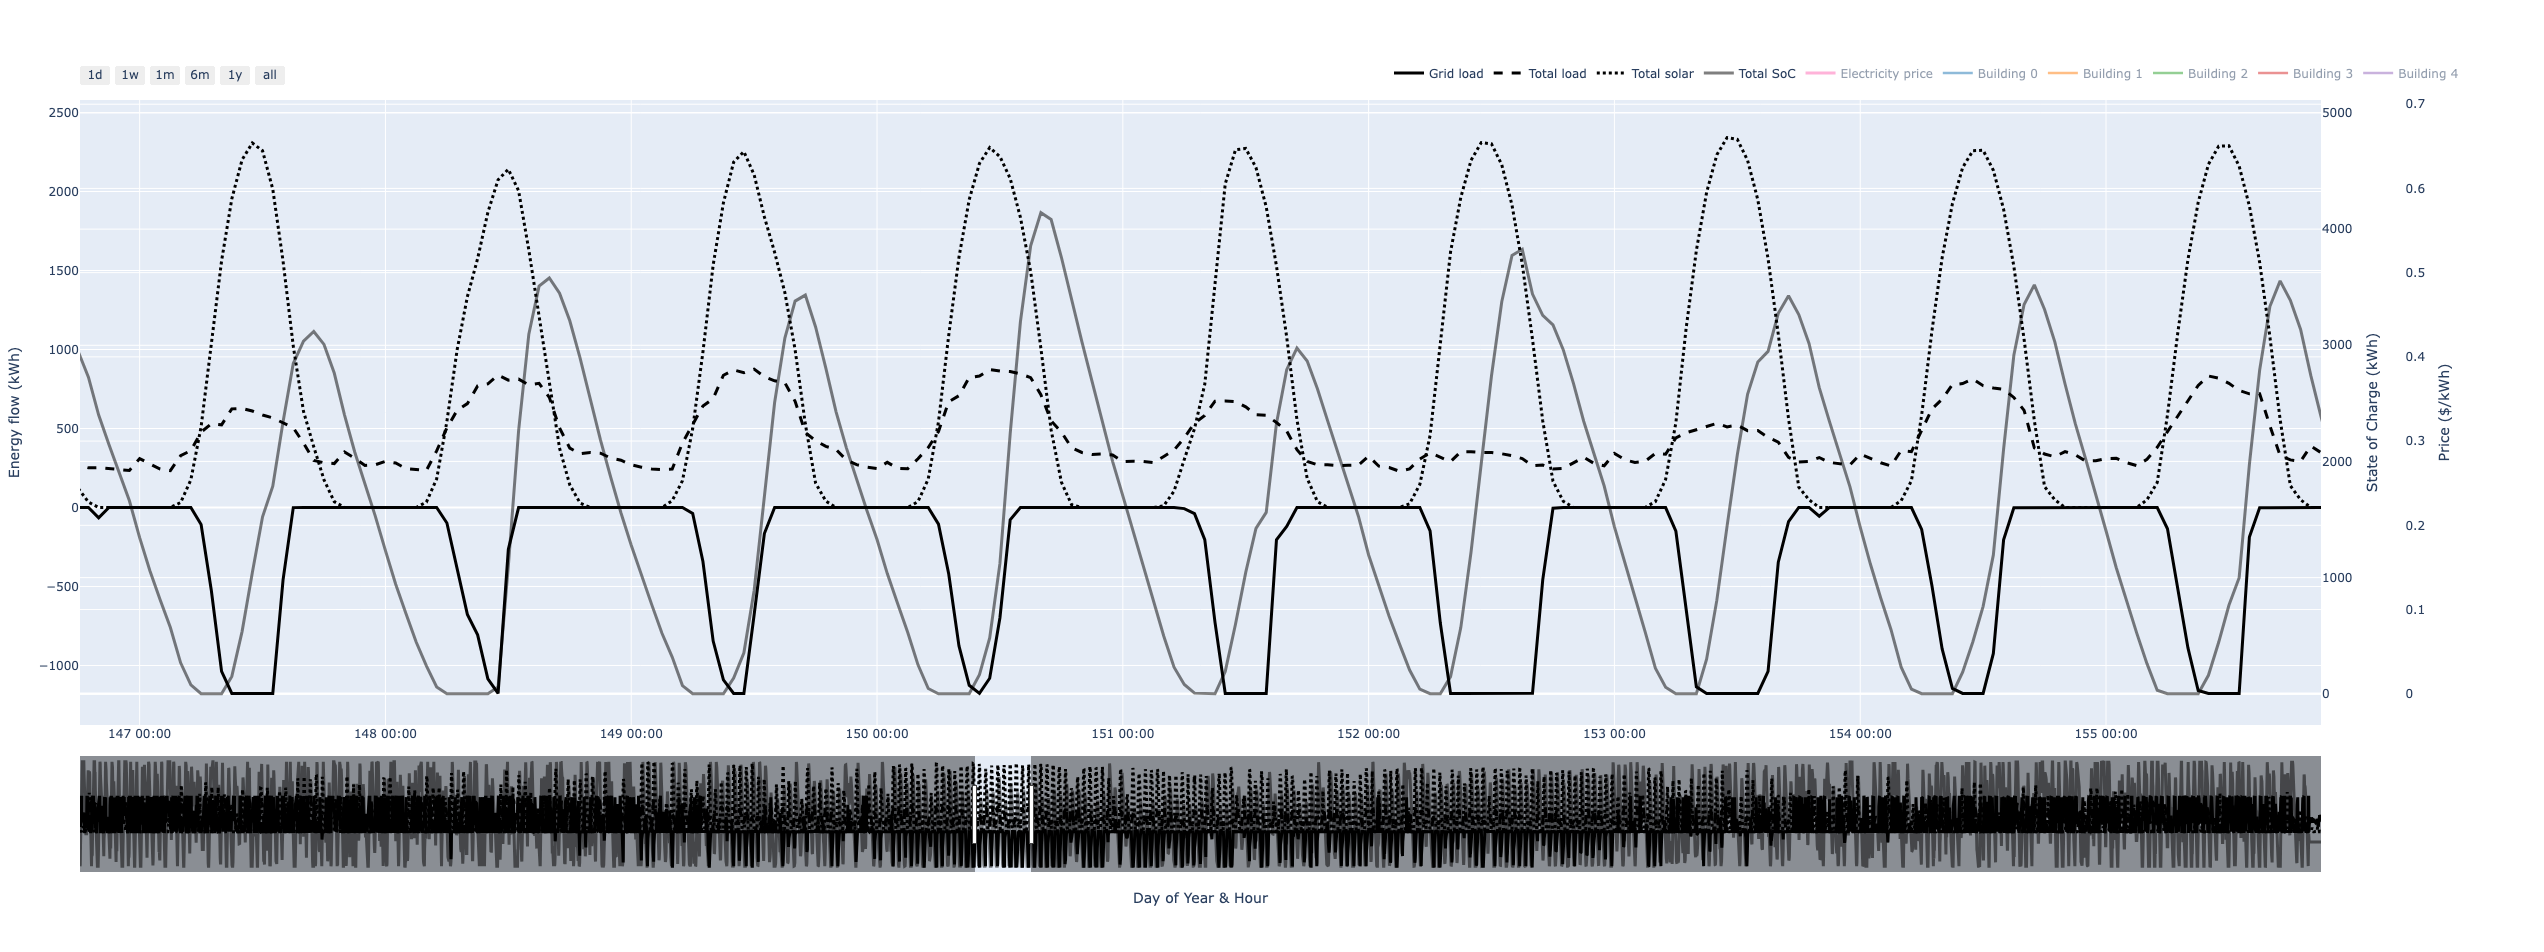
\includegraphics[width=\linewidth]{districts_prior-sim-summer.png}
                \label{fig:districts-prior-simulation-summer}
            }

            \subfloat[Winter.]{
                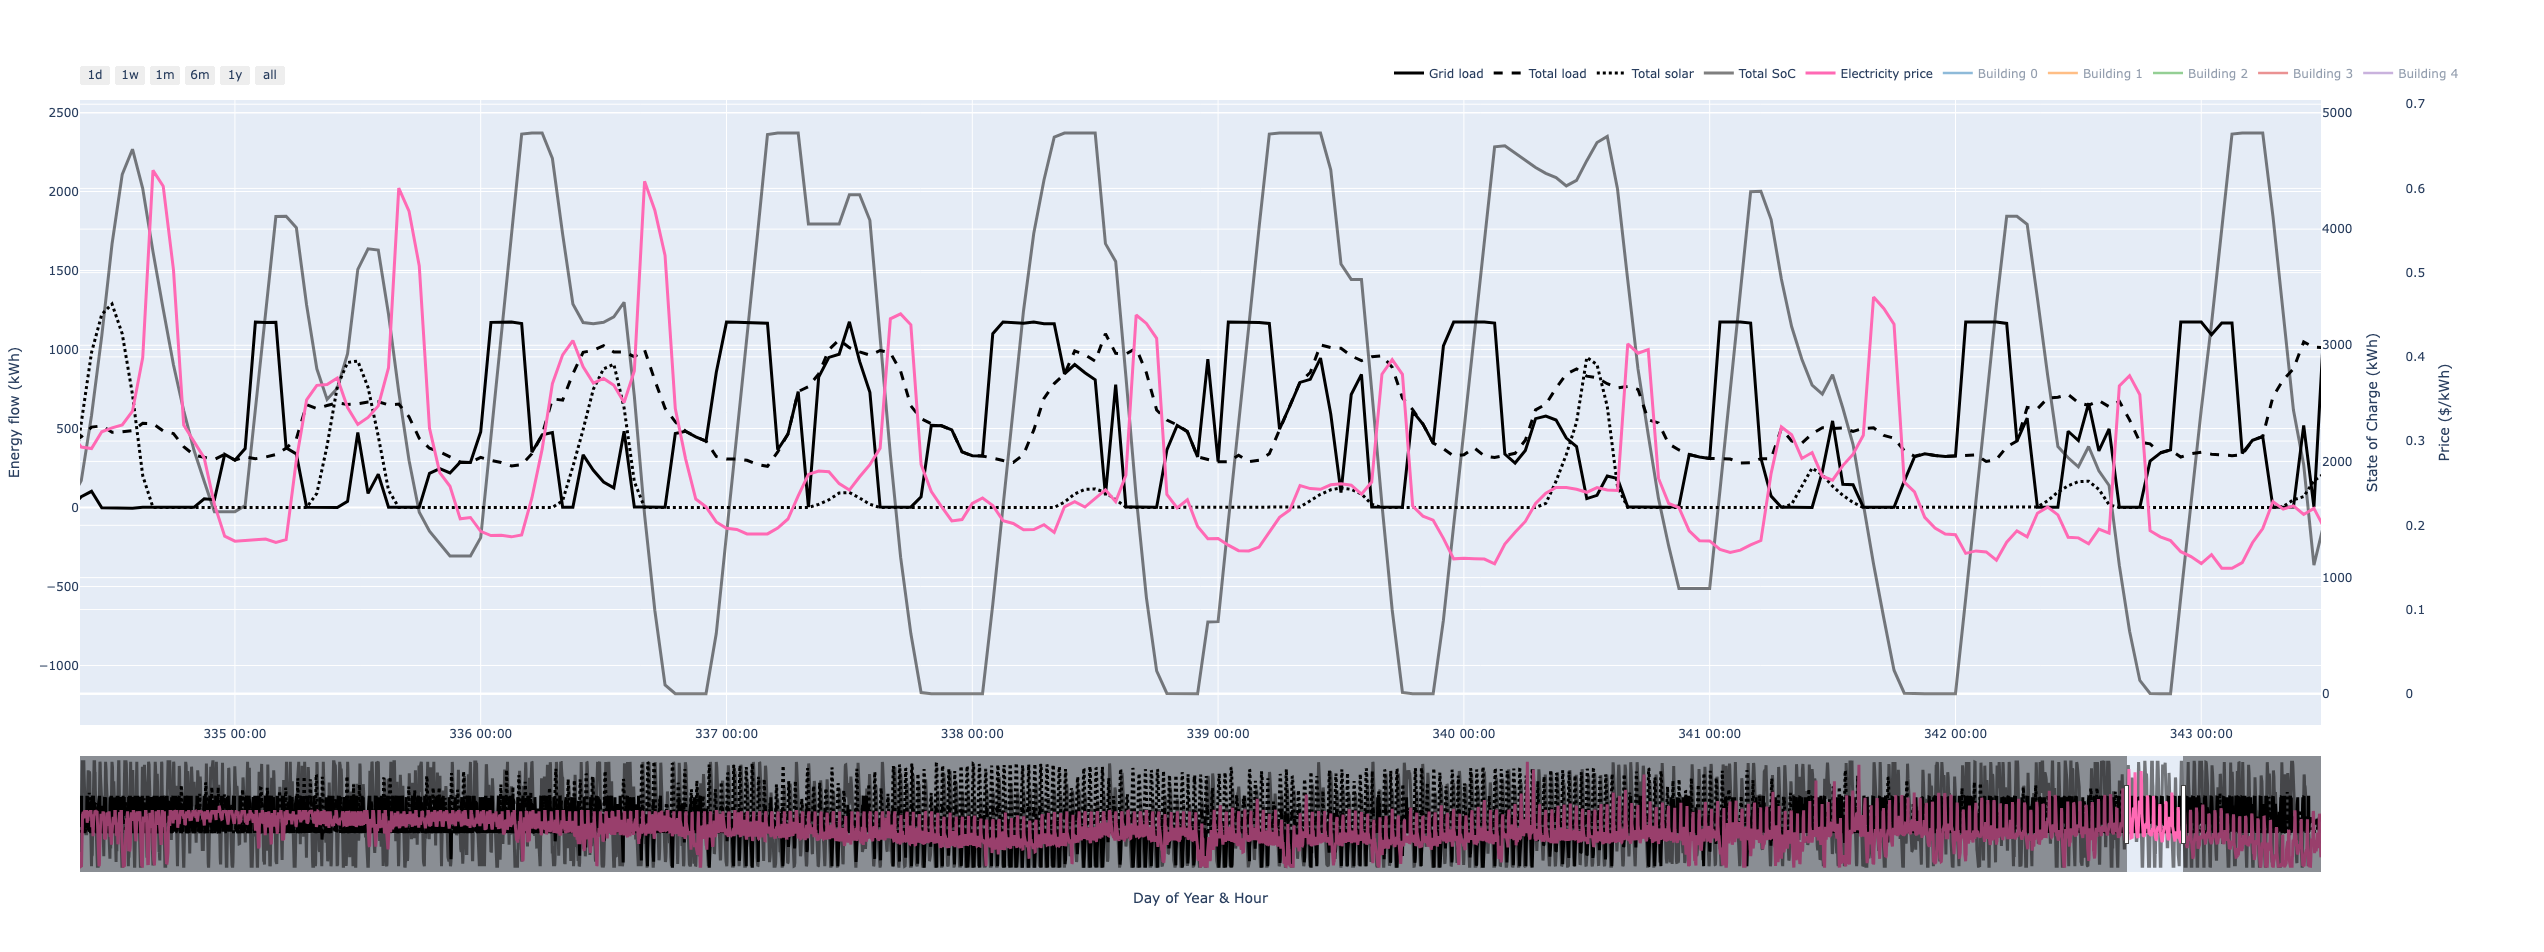
\includegraphics[width=\linewidth]{districts_prior-sim-winter.png}
                \label{fig:districts-prior-simulation-winter}
            }
            \vspace*{-0.2cm}
            \caption{Illustration of operation of prior system across seasons.}
            \label{fig:districts-prior-simulation}
            % add link to interactive example control plot
            \vspace{0.1cm}
            \small{\textit{Interactive version of plot available online} \href{https://mal84emma.github.io/Building-Design-VoI/example_prior_system_simulation.html}{\textbf{here}}.}
        \end{minipage}
    \end{figure}

    Observation of the operational behaviour of the district energy system provides insight into the factors driving system design. Fig. \ref{fig:districts-prior-simulation} plots the overall loads and battery state-of-charge in the district when operating over periods in both the summer (Fig. \ref{fig:districts-prior-simulation-summer}) and the winter (Fig. \ref{fig:districts-prior-simulation-winter}) for one of the sampled load scenarios. Readers can investigate the operational behaviour of the district energy system further using an interactive version of plot available online at \url{https://mal84emma.github.io/Building-Design-VoI/example_prior_system_simulation.html}.

    Comparing Figs \ref{fig:districts-prior-simulation-summer} \& \ref{fig:districts-prior-simulation-winter} shows that the net peak powers caused by local solar generation in the summer are significantly larger than those caused by building load in the winter. As a result, in the base case without constraints on the solar capacity, the required grid connection capacity is determined by the quantity of solar PV, and the optimization trades-off grid connection cost with additional cheap, zero-carbon solar energy. This implies that consideration of uncertainty in solar generation in the design optimization is important, as the capacity factor of solar generation will determine the scaling of this trade-off (noting that the peak power is well known as it is approximately the capacity in all years). This behaviour of the district energy system regularly exporting large quantities of energy onto the grid at around noon in the summer may cause issues for regulation of the power grid, as discussed in \citep{iweh2021DistributedGenerationRenewable}, and will require either adaptation of grid infrastructure to handle reverse power flow, or differentiated pricing for grid export capacity to discourage energy prosumers (customers with local generation) from flooding the grid with solar energy at these peak times. This may then increase the need for local storage to prevent surges in grid export to manage grid stability.

    For the majority of the summer, the district draws no power from the grid, though it provides significant quantities of energy to the grid. Therefore, over the summer this district would have zero energy bills. Additionally, as in this model the energy system operator is not paid for supplying energy to the grid, the solar generation capacity is therefore being set by its ability to provide cheap, zero-carbon energy during the spring and autumn to offset grid electricity. It is therefore correlated with the district mean load, as this determines the quantity of energy which must be offset. In future energy systems with large quantities of solar generation, it is likely that during peak generation times the price of grid electricity would fall to approximately zero, or potentially negative, as instantaneous generation exceeds energy demand.

    Full depth battery charge cycles are observed in the winter but not in the summer. This indicates that the battery capacities are determined by the financial benefit of arbitraging cheap grid electricity for use by the buildings at peak times. These capacities are then sufficient for maximising the usage of local solar energy generation, and managing power peaks to avoid exceeding the grid connection capacity. Fig. \ref{fig:districts-prior-simulation-winter} shows that the Model Predictive Controller successfully performs this price arbitrage of energy. On most days of the simulation, the power draw from the grid is near zero at peak demand times (around 5pm). In fact, this distributed generation and storage system reverses the timing of the peaks as the controller is not directed to smooth power usage.

    As the district mean load determines the quantity of energy which must be arbitraged to reduce the cost of satisfying building loads at peak times, via the same mechanism as for solar capacity, the optimal battery capacity is therefore also determined by the district mean load. This justifies the correlation between optimized solar and battery capacities observed in Fig. \ref{fig:districts-posterior-designs}.

    \newpage


    \section{Investigation of numerical accuracy \& computational requirements} \label{app:districts-numerics}

    \subsection{Statistical accuracy}
    %% Show MC estimate convergence to verify statistical accuracy of expectations
    % Estimate converge well within no. of samples, so sufficient samples have been used
    % Improved sampling technqiues (MCMC variants) could be used to improve sample efficiency (no. of effective samples, e.g. from tails) and reduce computational cost
    % Also, we could probably get away with fewer samples and still have a decent error
    % Compare standard errors on prior & posteriors separately vs standard error on VoI (treating as a single mean); 2nd option seems much more reasonable given visual convergence

    As the \glsxtrshort{voi} is the difference between two expectations, the prior and pre-posterior expected utilities (see Eq. \ref{eq:evii}), which are estimated using Monte Carlo sampling, the computed \glsxtrshort{voi} values are statistical estimates of some underlying true value. The statistical accuracy of these estimates must therefore be considered before firm conclusions can be drawn regarding whether data collection is worthwhile.

    Fig. \ref{fig:districts-MC-convergence} plots the convergence of the prior and pre-posterior expected utility estimates, as well as the \glsxtrshort{voi} estimate, as the number of samples from the building load distribution (scenarios, with corresponding designs and simulations) used increases. It also plots 95\% confidence intervals for the expectations using the standard error on the sample mean. For the \glsxtrshort{voi} estimate, the \glsxtrshort{voi} is considered as a single expectation, and the standard error is computed for the convergent sequence of \glsxtrshort{voi} estimates. The expectation estimates are seen to converge within the 256 samples used in the experiments, providing very similar estimates for all metrics after only 128 samples. This indicates that the \glsxtrshort{voi} values computed in the experiments have sufficient statistical accuracy to support the hypothesis that the \glsxtrshort{voi} is smaller than the cost of measurement, and therefore building monitoring is not financially worthwhile for supporting system design.

    \begin{figure}[h] % bounds are P95 (1.96sd)
        \centering
        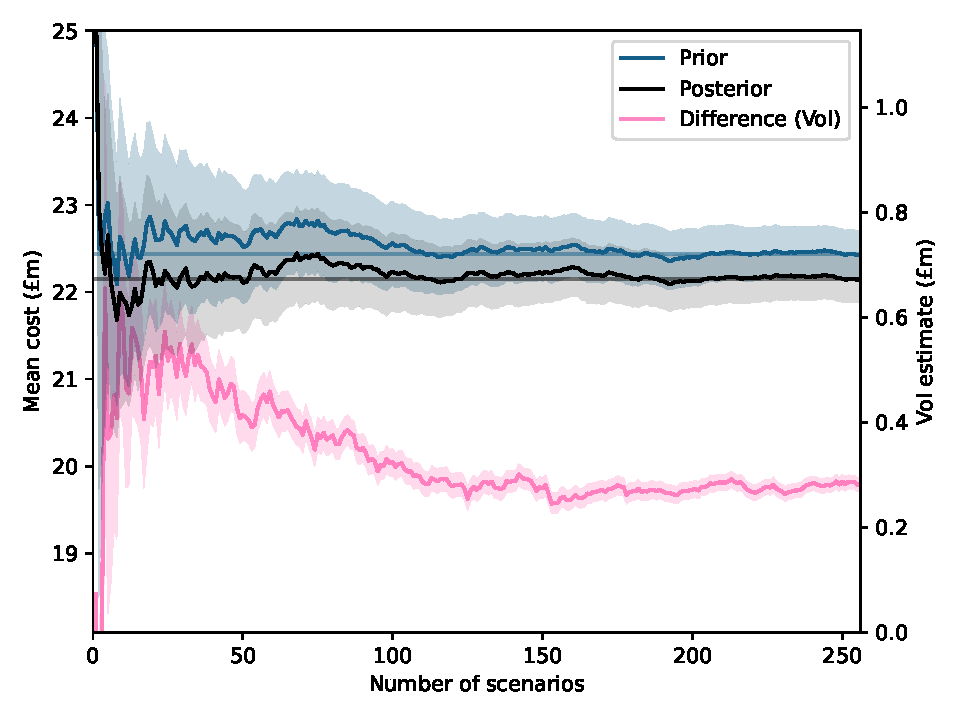
\includegraphics[width=0.66\linewidth]{districts_MC_conv.pdf}
        \caption{Convergence of \glsxtrlong{mc} estimates of expected utilities with number of samples from building load distribution.}
        \label{fig:districts-MC-convergence}
    \end{figure}

    In this study a naive sampling scheme was used to sample from the building load distribution. The use of improved sampling techniques which provide greater sample efficiency for the load distribution would speed up the convergence of the expectation estimates, and so reduce the computational cost of achieving sufficient statistical accuracy in the \glsxtrshort{voi} estimates. Further work is required to properly quantify the statistical error of \glsxtrshort{voi} estimates, and develop techniques for determining the number of samples required to achieve sufficient statistical accuracy to support conclusions drawn from the \glsxtrshort{voi}, i.e. whether it is greater or less than some cost threshold. Such developments are necessary to reduce the computational cost of \glsxtrshort{voi} calculations, to allow the study of complex, practical engineering decision problems, whilst providing confidence that the data collection strategy recommendations they produce are correct with high probability.

    \subsection{Cost estimation accuracy} \label{app:districts-cost-accuracy}
    %% Discuss accuracy of SP objectives - surprisingly good with only 10 scenarios and extremely simple scenario reduction (also the case for 1 building?) - but this couldn't be known a priori
    % Briefly compare SP objectives to evals and comment on gap (very small gap considering no. of SP scenarios) - discuss why (little planning benefit from more than 48hrs of foresight as energy storage only for short durations)
    % We claimed that the SP objective *may* not be a good approximation of the actual cost and could obscure the VoI - check this (for both prior & posterior SPs); initial checks seem to suggest objective is very good approximation for 2 reasons: 1 very little intra-day storage interaction (so perfect foresight provides little benefit), grid cap FoS well calibrated (very small grid excess charges in operation) => for this case could get rid of utility eval step and save lots of computation; this is actually quite impressive considering such basic scenario reduction is used as well as only 10 MC samples for objective
    % Discuss practical importance for buiding design using SPs and the trustworthiness of their cost predictions - obviously limitation is that we used perfect foresight, and practical forecasts lead to worse performance, as demonstrated in Annex paper (cite)
    % Removing simulation step would save c. 80% of runtime and make VoI calculations far more achievable, i.e. 100 LPs could be solved in parallel on HPC

    The On-Policy \glsxtrshort{voi} framework proposed in \Cref{sec:methodology-on-policy-voi} enables the \glsxtrshort{voi} to be computed for complex decision problems where policies which do not necessarily provide an accurate estimate of the decision utility must be used for computational tractability. For the case study considered in this work, Stochastic Programming (SP) is needed to optimize the energy system sizing as the number of decision variables and simulation time make the application of stochastic global optimization methods directly to the simulator intractable. However, the SP's estimate of mean system cost (expected utility) suffers from two sources of inaccuracy.

    Firstly, the SP can only include 10 scenarios in its Monte Carlo estimate of mean operational cost within its objective function to run in a manageable computation time. This leads to potentially significant statistical error in the estimate of cost that is minimized. An attempt is made to manage this by using scenario reduction to select the 10 samples/scenarios that provide the best statistical representation of the population. However, as the space of possible load profiles is extremely large, only simple summary statistics could be used as the targeted statistical metric to represent, meaning the selection of scenarios to include in the SP does not have a direct link to the distribution of operational costs. Secondly, modelling error is introduced as the Linear Program formulation of the decision problem requires the assumption that the energy system is controlled with perfect foresight of the operational conditions, i.e. the weather and electricity price are known perfectly for all future periods during control. This assumption is not realistic and can lead to the SP model underestimating operational costs as the system is able to pre-empt difficult operational conditions and make unrealistically good control decisions in advance to reduce overall cost. In the case of managing the grid impact of energy usage under load uncertainty this assumption can be particularly over-optimistic, as unforeseen load conditions can lead to the battery state-of-charge not being sufficient to manage large peak loads, leading to substantial grid excess charges. Assuming perfect foresight allows the system to manage the battery level to avoid these instances, and causes a significant underestimate of operational cost. In fact, it is this over-optimism regarding the system's ability to manage peak loads that leads to the need to include a factor-of-safety on grid capacity during design.

    Therefore, as these model and statistical errors could lead to significant inaccuracy in the SP's estimate of operating costs, a simulation step was included to provide a more accurate estimate of the true costs. These simulations used a Model Predictive Controller with only 48 hours of perfect foresight\footnotemark, and evaluated a large number of sampled load scenarios to overcome both the model and statistical inaccuracies.
    \footnotetext{This controller is still unrealistic, as perfect foresight even over a limited planning horizon leads to practically unachievably low operational costs, as demonstrated in \citep{langtry2024ImpactDataForecasting}. While it would not be feasible to train practical prediction algorithms to use in each simulation, a controller using synthetically noisy forecasts calibrated to the properties of practical forecasting methods could be used to improve the realism of the simulated operation and resulting costs.}

    The accuracy of the Stochastic Program model objective was investigated by comparing it to the mean system operating costs determined by simulation. Table \ref{tab:districts-SP-obj-error} provides both the mean error and mean absolute error of the SP objective for system designs performed with both the prior and posterior distributions, across the range of cases considered in the experiments. Fig. \ref{fig:districts-post-SP-obj-error} plots the distribution of objective errors for  the SP designs performed for each measurement scenario in the base case, where all uncertainties were reduced.

    \begin{table}[h]
        \centering
        \renewcommand{\arraystretch}{1}
        \begin{tabular}{c|cc} \toprule \toprule
            Case & Mean error (\%) & Mean absolute error (\%) \\
            \midrule \midrule
            \multicolumn{3}{>{\centering\arraybackslash}l}{\footnotesize \qquad Prior cases (as considered in \Cref{sec:districts-alt-systems}) - point estimates} \\[1ex]
            Base & -0.345 & 0.345 \\
            Solar constrained & -0.423 & 0.423 \\
            1 building & -3.062 & 3.062 \\
            \midrule
            \multicolumn{3}{>{\centering\arraybackslash}l}{\footnotesize \qquad Posterior cases (as defined in Table \ref{tab:districts-VOI-contributions} of \Cref{sec:districts-contributions}) - av. over 256 msrmnts.} \\[1ex]
            \texttt{type} & 0.683 & 0.811 \\
            \texttt{peak} & -0.113 & 0.899 \\
            \texttt{mean} & -0.633 & 1.052 \\
            All (base) & -0.271 & 0.525 \\
            \bottomrule \bottomrule
        \end{tabular}
        \smallskip
        \caption{Errors in SP estimates of mean system operating costs for optimized designs (under-estimation +ve).}
        \label{tab:districts-SP-obj-error}
    \end{table}

    \begin{figure}[h]
        \centering
        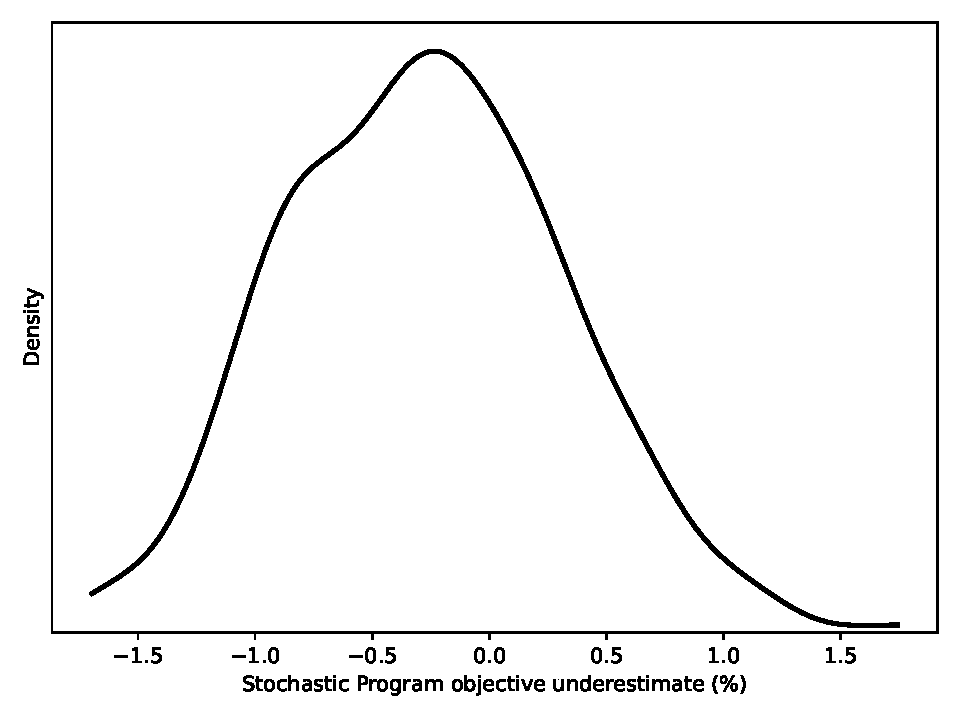
\includegraphics[width=0.75\linewidth]{districts_post_SP_obj_error.pdf}
        \caption{Distribution of Stochastic Program objective value errors compared to simulated mean operating costs for posterior designs in base case.}
        \label{fig:districts-post-SP-obj-error}
    \end{figure}

    The results show that the Stochastic Program is able to estimate the mean operating cost within around 0.25-1\% (except for the single building case where the error is significantly higher), and in fact more frequently over-estimates the cost than under-estimates. This result is somewhat surprising considering that only 10 scenarios are considered in the SP objective, and these scenarios were selected in a simplistic manner. From the plots of operational behaviour (Fig. \ref{fig:districts-prior-simulation}) it can be seen that battery charge is rarely held for more than 72 hours, which indicates that during operation, assumption of complete perfect foresight would not lead to significant under-estimation of operational costs. However, this also demonstrates that the factor-of-safety used during design is performing well as the system does not end up in situations where it does not have the state-of-charge needed to manage peak loads. Additionally, as district mean load was one of the metrics used in scenario reduction, and was found to be the key driver of operational cost (\Cref{sec:districts-prior-design}), the scenario reduction was able to well represent the distribution of costs through correlation.

    However, whilst the SP objective error is relatively low, it is approximately the same magnitude as the \glsxtrshort{voi}, which was 1.27\% in the base case. An additional 1\% cost error added to the \glsxtrshort{voi} estimate could have led to the conclusion that building monitoring was economically worthwhile, as it would have put it at around the same level as the estimated cost of performing the measurement. However, the impact of the SP objective error on the \glsxtrshort{voi} estimate is complex, as it depends on the error in the difference between the prior and pre-posterior cost estimates, which is challenging to study. Ultimately, verifying that the error is sufficiently low may be as computationally expensive as performing the simulations required by the On-Policy \glsxtrshort{voi} calculation.


    \subsection{Computational cost}

    The computational cost of the experiments performed in this study was very large, with each \glsxtrshort{voi} calculation taking roughly 10 days of computation time on a powerful desktop workstation\footnote{32 core, 2.90 GHz Intel Xeon Gold CPU with 256 GB of DDR4 RAM.} with a parallel processing workflow. Performing the simulations took approximately 80\% of runtime.

    Reducing the number of samples required by the Monte Carlo estimates of expected utilities, or removing the need for simulation to accurately estimate utilities, would greatly decrease the computational cost of \glsxtrshort{voi} calculations.
    Given that the SP objectives are found to be reasonably accurate estimates of the simulator costs in \ref{app:districts-cost-accuracy}, a good estimate of the \glsxtrshort{voi} could be obtained in only 20\% of the original runtime.
    A key advantage of \glsxtrshort{voi} calculations is that they are highly parallelizable, as each scenario can be evaluated independently, making them well suited for distributed computation. I.e. the optimization based design and simulator evaluation can be performed simultaneously for each measurement scenario, meaning the computation time can be drastically reduced if sufficient compute resources are available.

\end{subappendices}